\label{2.5 C7M Answer Key}
\subsection{Answer Key}
\tiny
\renewcommand{\insertclass}{- Class 7}
\renewcommand{\insertsubject}{ - Math}

\begin{frame}[shrink=0.1,label=QPC7QC6M04 - BM - Q1]{Q1 [Basic Math]}
\vspace{-0.2cm}
\mcqtextbottomOneFour{
  questionnumber={1}, 
  questionTag={C6M04 - BM - Q1}, 
  questiontext={Find the least common multiple for 42, 84},
  optionA={84},
  optionB={42},
  optionC={40},
  optionD={2},
  correctoption={A},
}

\begin{minipage}{\linewidth}
\hspace{1cm}
\centering
\tiny
\renewcommand{\arraystretch}{1.25}
\begin{tabular}{|M{1.2cm}|M{0.8cm}|M{0.8cm}|M{0.8cm}|M{0.8cm}|M{0.8cm}|}
\hline
Option & \cellcolor{cellgreen} A (\ding{51}) & B (\ding{55}) & C (\ding{55}) & D (\ding{55}) & E \\ 
\hline
7 A & \highred{25\%} & \highno{25\%} & \highno{0\%} & \highno{50\%} & \highno{0\%} \\ 
 \hline 
7 B & \highred{29\%} & \highno{21\%} & \highno{0\%} & \highno{43\%} & \highno{7\%} \\ \hline
\end{tabular}
\end{minipage}

\end{frame}
% \input{4. PPT/My Answer/Math/C7/117_C7M - Q1}


\begin{frame}[shrink=0.1,label=QPC7QC5BM - BM - Q9]{Q2 [Basic Math]}
\vspace{-0.2cm}
\mcqimgleftFourOne{
  questionnumber={2}, 
  questionTag={C5BM - BM - Q9},
  questiontext={Find the quotient in the following division.},
  imgtabletikz = {
  \begin{table}[H]
      \centering
      \renewcommand{\arraystretch}{1}
      \begin{tabular}{c|cccccc}
           \multicolumn{1}{c}{}  & & ? &  & &$\longrightarrow$ & Quotient  \\
           \cline{2-5}
           6 & & 3 & 6 & 6   \\
          \multicolumn{1}{c}{} & $-$ & 3 & 6 && &  \\
           \cline{2-5}
            \multicolumn{1}{c}{} & & & 0 & 6 & & \\
           \multicolumn{1}{c}{} & $-$ & & & 6 & & \\
           \cline{2-5}
            \multicolumn{1}{c}{} & &  &0& & $\longrightarrow$ & Remainder  \\
            \cline{2-5}
      \end{tabular}
  \end{table} },
  optionA={36},
  optionB={366},
  optionC={61},
  optionD={66},
  correctoption={C},
  leftmini={0.5},
  rightmini={0.4},
}

\begin{minipage}{\linewidth}
\hspace{1cm}
\centering
\tiny
\renewcommand{\arraystretch}{1.25}
\begin{tabular}{|M{1.2cm}|M{0.8cm}|M{0.8cm}|M{0.8cm}|M{0.8cm}|M{0.8cm}|}
\hline
Option & A (\ding{55}) & B (\ding{55}) & \cellcolor{cellgreen} C (\ding{51}) & D (\ding{55}) & E \\ 
\hline
7 A & \highno{0\%} & \highno{0\%} & \highgreen{100\%} & \highno{0\%} & \highno{0\%} \\ 
 \hline 
7 B & \highno{7\%} & \highno{0\%} & \highgreen{86\%} & \highno{0\%} & \highno{7\%} \\ \hline
\end{tabular}
\end{minipage}

\end{frame}
% \input{4. PPT/My Answer/Math/C7/117_C7M - Q2}


\begin{frame}[shrink=0.1,label=QPC7QC6M01 - BM - Q5]{Q3 [Basic Math]}
\vspace{-0.2cm}
\mcqimgleftFourOne{
  questionnumber={3}, 
  questionTag={C6M01 - BM - Q5},
  questiontext={Subtract.},
  imgtabletikz = {
  \begin{table}[H]
      \centering
      \renewcommand{\arraystretch}{1.5}
      \begin{tabular}{ccccccc}
           &1 &5 &6 &7 &5 &9  \\
          ($-$) &&1&2&3&6&7 \\
          \hline
          &&&&&&\\
          \hline
      \end{tabular}
  \end{table}
  },
  optionA={12389},
  optionB={33089},
  optionC={144392},
  optionD={144312},
  correctoption={C},
  leftmini={0.5},
  rightmini={0.4},
}

\begin{minipage}{\linewidth}
\hspace{1cm}
\centering
\tiny
\renewcommand{\arraystretch}{1.25}
\begin{tabular}{|M{1.2cm}|M{0.8cm}|M{0.8cm}|M{0.8cm}|M{0.8cm}|M{0.8cm}|}
\hline
Option & A (\ding{55}) & B (\ding{55}) & \cellcolor{cellgreen} C (\ding{51}) & D (\ding{55}) & E \\ 
\hline
7 A & \highno{0\%} & \highno{0\%} & \highgreen{94\%} & \highno{6\%} & \highno{0\%} \\ 
 \hline 
7 B & \highno{0\%} & \highno{7\%} & \highgreen{86\%} & \highno{0\%} & \highno{7\%} \\ \hline
\end{tabular}
\end{minipage}

\end{frame}
% \input{4. PPT/My Answer/Math/C7/117_C7M - Q3}


\begin{frame}[shrink=0.1,label=QPC7QC6M01 - BM - Q1]{Q4 [Basic Math]}
\vspace{-0.2cm}
\mcqtextbottomOneFour{
  questionnumber={4}, 
  questionTag={C6M01 - BM - Q1}, 
  questiontext={Fill in the blanks.\\
  \qquad i.  1 cm = \rule{40pt}{0.5pt} m \qquad ii. 1 kg = \rule{40pt}{0.5pt} g},
  optionA={100 m, 1000 g },
  optionB={1000 m, 0.001 g },
  optionC={0.0001 m, 100 g },
  optionD={0.01 m, 1000 g},
  correctoption={D},
}

\begin{minipage}{\linewidth}
\hspace{1cm}
\centering
\tiny
\renewcommand{\arraystretch}{1.25}
\begin{tabular}{|M{1.2cm}|M{0.8cm}|M{0.8cm}|M{0.8cm}|M{0.8cm}|M{0.8cm}|}
\hline
Option & A (\ding{55}) & B (\ding{55}) & C (\ding{55}) & \cellcolor{cellgreen} D (\ding{51}) & E \\ 
\hline
7 A & \highno{38\%} & \highno{6\%} & \highno{6\%} & \highno{44\%} & \highno{6\%} \\ 
 \hline 
7 B & \highno{57\%} & \highno{0\%} & \highno{0\%} & \highno{43\%} & \highno{0\%} \\ \hline
\end{tabular}
\end{minipage}

\end{frame}
% \input{4. PPT/My Answer/Math/C7/117_C7M - Q4}


\begin{frame}[shrink=0.1,label=QPC7QC6M04 - BM - Q2]{Q5 [Basic Math]}
\vspace{-0.2cm}
\mcqtextbottomOneFour{
  questionnumber={5}, 
  questionTag={C6M04 - BM - Q2}, 
  questiontext={Find the prime factorization of 45.},
  optionA={3 $\times$ 3 $\times$ 5},
  optionB={3 $\times$ 5 $\times$ 5},
  optionC={9 $\times$ 5},
  optionD={3 $\times$ 3},
  correctoption={A},
}

\begin{minipage}{\linewidth}
\hspace{1cm}
\centering
\tiny
\renewcommand{\arraystretch}{1.25}
\begin{tabular}{|M{1.2cm}|M{0.8cm}|M{0.8cm}|M{0.8cm}|M{0.8cm}|M{0.8cm}|}
\hline
Option & \cellcolor{cellgreen} A (\ding{51}) & B (\ding{55}) & C (\ding{55}) & D (\ding{55}) & E \\ 
\hline
7 A & \highno{69\%} & \highno{0\%} & \highno{31\%} & \highno{0\%} & \highno{0\%} \\ 
 \hline 
7 B & \highno{71\%} & \highno{0\%} & \highno{29\%} & \highno{0\%} & \highno{0\%} \\ \hline
\end{tabular}
\end{minipage}

\end{frame}
% \input{4. PPT/My Answer/Math/C7/117_C7M - Q5}


\begin{frame}[shrink=0.1,label=QPC7QC7M01 - DT - Q2]{Q37 [1. Integers]}
\vspace{-0.2cm}
\mcqtextbottomOneFour{
  questionnumber={37}, 
  questionTag={C7M01 – DT – Q2}, 
  questiontext={\rule{80pt}{0.1pt} are the set of whole numbers along with negative numbers.},
  optionA={Negative integers},
  optionB={Positive numbers},
  optionC={Integers},
  optionD={Natural numbers},
  correctoption={C},
}

\begin{minipage}{\linewidth}
\hspace{1cm}
\centering
\tiny
\renewcommand{\arraystretch}{1.25}
\begin{tabular}{|M{1.2cm}|M{0.8cm}|M{0.8cm}|M{0.8cm}|M{0.8cm}|M{0.8cm}|}
\hline
Option & A (\ding{55}) & B (\ding{55}) & \cellcolor{cellgreen} C (\ding{51}) & D (\ding{55}) & E \\ 
\hline
7 A & \highno{19\%} & \highno{6\%} & \highno{63\%} & \highno{13\%} & \highno{0\%} \\ 
 \hline 
7 B & \highno{14\%} & \highno{29\%} & \highno{43\%} & \highno{14\%} & \highno{0\%} \\ \hline
\end{tabular}
\end{minipage}

\end{frame}
% \input{4. PPT/My Answer/Math/C7/117_C7M - Q37}


\begin{frame}[shrink=0.1,label=QPC7QC7M01 - DT - Q5]{Q39 [1. Integers]}
\vspace{-0.2cm}
\mcqtextbottomOneFour{
  questionnumber={39}, 
  questionTag={C7M01 – DT – Q5}, 
  questiontext={Find the option that results in a negative integer.},
  optionA={ $-$3 $\divisionsymbol$ ($-$3)},
  optionB={  3 $\divisionsymbol$ (3)},
  optionC={ $-$3 $\divisionsymbol$ (3)},
  optionD={Both a and b},
  correctoption={C},
}

\begin{minipage}{\linewidth}
\hspace{1cm}
\centering
\tiny
\renewcommand{\arraystretch}{1.25}
\begin{tabular}{|M{1.2cm}|M{0.8cm}|M{0.8cm}|M{0.8cm}|M{0.8cm}|M{0.8cm}|}
\hline
Option & A (\ding{55}) & B (\ding{55}) & \cellcolor{cellgreen} C (\ding{51}) & D (\ding{55}) & E \\ 
\hline
7 A & \highno{13\%} & \highno{6\%} & \highno{75\%} & \highno{6\%} & \highno{0\%} \\ 
 \hline 
7 B & \highno{14\%} & \highno{7\%} & \highno{64\%} & \highno{14\%} & \highno{0\%} \\ \hline
\end{tabular}
\end{minipage}

\end{frame}
% \input{4. PPT/My Answer/Math/C7/117_C7M - Q39}


\begin{frame}[shrink=0.1,label=QPC7QC7M01 - DT - Q4]{Q48 [1. Integers]}
\vspace{-0.2cm}
\mcqtextbottomOneFour{
  questionnumber={48}, 
  questionTag={C7M01 – DT – Q4}, 
  questiontext={Multiply: \quad i. $-$10 $\times$ 0 
  \qquad ii. $-$5 $\times$ $-$10},
  optionA={$-$10, $-$15},
  optionB={$-$0, $-$50},
  optionC={0, 50},
  optionD={1, $-$50},
  correctoption={C},
}

\begin{minipage}{\linewidth}
\hspace{1cm}
\centering
\tiny
\renewcommand{\arraystretch}{1.25}
\begin{tabular}{|M{1.2cm}|M{0.8cm}|M{0.8cm}|M{0.8cm}|M{0.8cm}|M{0.8cm}|}
\hline
Option & A (\ding{55}) & B (\ding{55}) & \cellcolor{cellgreen} C (\ding{51}) & D (\ding{55}) & E \\ 
\hline
7 A & \highno{0\%} & \highno{13\%} & \highgreen{81\%} & \highno{0\%} & \highno{6\%} \\ 
 \hline 
7 B & \highno{0\%} & \highno{21\%} & \highgreen{79\%} & \highno{0\%} & \highno{0\%} \\ \hline
\end{tabular}
\end{minipage}

\end{frame}
% \input{4. PPT/My Answer/Math/C7/117_C7M - Q48}


\begin{frame}[shrink=0.1,label=QPC7QC7M03 - DT - Q1]{Q9 [2. Fractions and Decimals]}
\vspace{-0.2cm}
\mcqtextbottomOneFour{
  questionnumber={9}, 
  questionTag={C7M03 – DT – Q1}, 
  questiontext={Identify the place value of 6 in 1234.4568},
  optionA={Ones},
  optionB={Oneth},
  optionC={Hundredth},
  optionD={Thousandth},
  correctoption={D},
}

\begin{minipage}{\linewidth}
\hspace{1cm}
\centering
\tiny
\renewcommand{\arraystretch}{1.25}
\begin{tabular}{|M{1.2cm}|M{0.8cm}|M{0.8cm}|M{0.8cm}|M{0.8cm}|M{0.8cm}|}
\hline
Option & A (\ding{55}) & B (\ding{55}) & C (\ding{55}) & \cellcolor{cellgreen} D (\ding{51}) & E \\ 
\hline
7 A & \highno{6\%} & \highno{50\%} & \highno{44\%} & \highred{0\%} & \highno{0\%} \\ 
 \hline 
7 B & \highno{7\%} & \highno{29\%} & \highno{29\%} & \highred{21\%} & \highno{14\%} \\ \hline
\end{tabular}
\end{minipage}

\end{frame}
% \input{4. PPT/My Answer/Math/C7/117_C7M - Q9}


\begin{frame}[shrink=0.1,label=QPC7QC7M03 - DT - Q5]{Q11 [2. Fractions and Decimals]}
\vspace{-0.2cm}
\mcqimgleftFourOne{
  questionnumber={11}, 
  questionTag={C7M03 – DT – Q5},
  questiontext={Ken bought two pens. The prices of the pens are given below. Find the total price of the pens.},
  imgtabletikz = { \adjustbox{scale=\scalefactor}{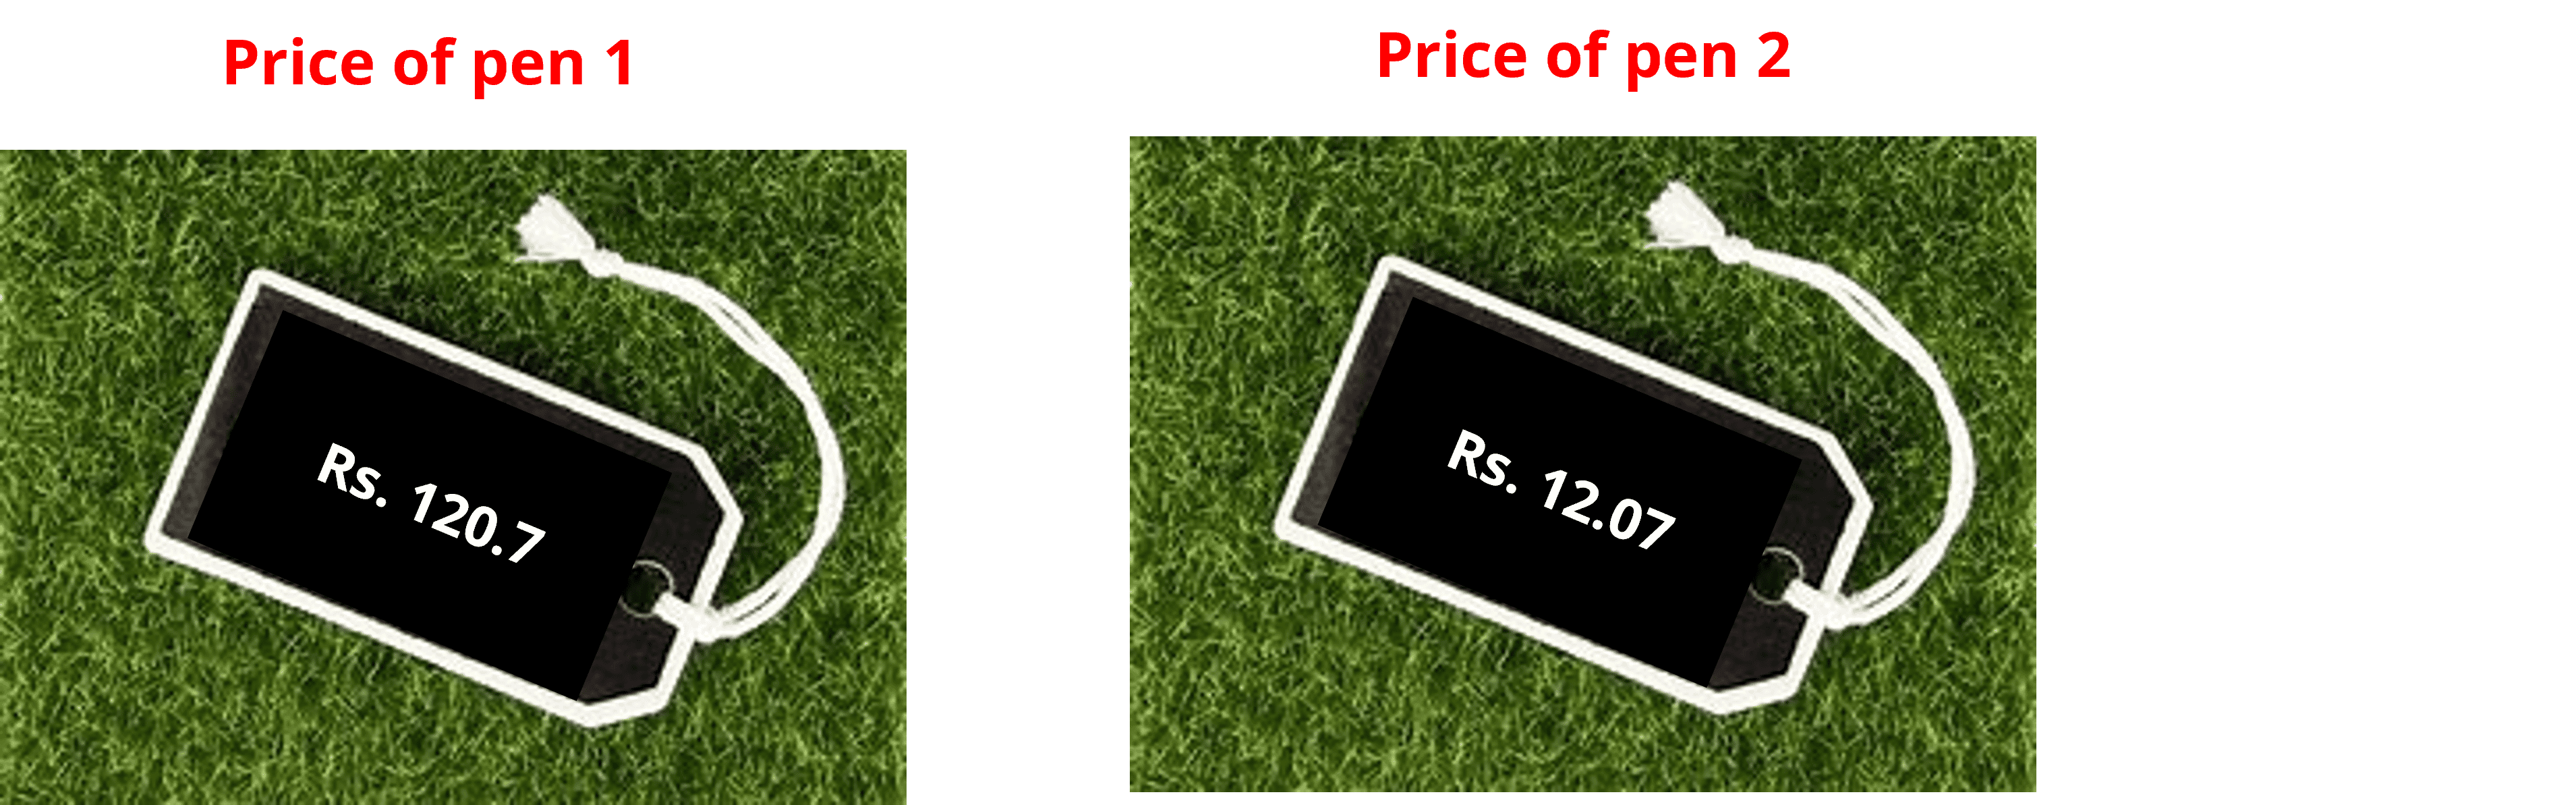
\includegraphics[width=11cm, height=3cm]{C7M03 - DT - Q5.png}} },
  optionA={Rs. 241.4},
  optionB={Rs. 24.14},
  optionC={Rs. 132.77},
  optionD={Rs. 240.14},
  correctoption={C},
  leftmini={0.5},
  rightmini={0.4},
}

\begin{minipage}{\linewidth}
\hspace{1cm}
\centering
\tiny
\renewcommand{\arraystretch}{1.25}
\begin{tabular}{|M{1.2cm}|M{0.8cm}|M{0.8cm}|M{0.8cm}|M{0.8cm}|M{0.8cm}|}
\hline
Option & A (\ding{55}) & B (\ding{55}) & \cellcolor{cellgreen} C (\ding{51}) & D (\ding{55}) & E \\ 
\hline
7 A & \highno{13\%} & \highno{0\%} & \highno{75\%} & \highno{13\%} & \highno{0\%} \\ 
 \hline 
7 B & \highno{7\%} & \highno{14\%} & \highno{64\%} & \highno{14\%} & \highno{0\%} \\ \hline
\end{tabular}
\end{minipage}

\end{frame}
% \input{4. PPT/My Answer/Math/C7/117_C7M - Q11}


\begin{frame}[shrink=0.1,label=QPC7QC7M03 - DT - Q6]{Q24 [2. Fractions and Decimals]}
\vspace{-0.2cm}
\mcqimgleftFourOne{
  questionnumber={24}, 
  questionTag={C7M03 – DT – Q6},
  questiontext={Match the expressions in column A with their decimal equivalents in column B.},
  imgtabletikz = {\renewcommand{\arraystretch}{1.25}
\begin{tabular}{|p{0.25cm}|p{3cm}|p{0.25cm}|p{0.25cm}|p{3cm}|}
\hline
\multicolumn{2}{|c|}{Column A} & & \multicolumn{2}{|c|}{Column B} \\
\cline{1-2}\cline{4-5}
 i & 0.2 $\times$ 2.5  & & a& 11.2 \\
\cline{1-2}\cline{4-5}
ii & 4.48 $\divisionsymbol$ 0.4 & & b & 5.5 \\
\cline{1-2}\cline{4-5}
iii & 5 {{$\dfrac{1}{2}$}} & & c& 0.5 \\
\hline
\end{tabular}
},
  optionA={i - a, ii - c, iii - b},
  optionB={i - b, ii - a, iii - c},
  optionC={i - c, ii - a, iii - b},
  optionD={i - c, ii - b, iii - a},
  correctoption={C},
  leftmini={0.6},
  rightmini={0.3},
}

\begin{minipage}{\linewidth}
\hspace{1cm}
\centering
\tiny
\renewcommand{\arraystretch}{1.25}
\begin{tabular}{|M{1.2cm}|M{0.8cm}|M{0.8cm}|M{0.8cm}|M{0.8cm}|M{0.8cm}|}
\hline
Option & A (\ding{55}) & B (\ding{55}) & \cellcolor{cellgreen} C (\ding{51}) & D (\ding{55}) & E \\ 
\hline
7 A & \highno{13\%} & \highno{25\%} & \highred{38\%} & \highno{25\%} & \highno{0\%} \\ 
 \hline 
7 B & \highno{0\%} & \highno{14\%} & \highno{50\%} & \highno{36\%} & \highno{0\%} \\ \hline
\end{tabular}
\end{minipage}

\end{frame}
% \input{4. PPT/My Answer/Math/C7/117_C7M - Q24}


\begin{frame}[shrink=0.1,label=QPC7QC7M02 - DT - Q3]{Q32 [2. Fractions and Decimals]}
\vspace{-0.2cm}
\mcqimgleftFourOne{
  questionnumber={32}, 
  questionTag={C7M02 – DT – Q3},
  questiontext={Identify the fraction of pizzas left in the box.},
  imgtabletikz = { \adjustbox{scale=\scalefactor}{
\includegraphics[width=4cm, height=4cm]{C7M02 – DT – Q3.png}} },
  optionA={{{$\dfrac{3}{3}$}}},
  optionB={{{$\dfrac{5}{3}$}}},
  optionC={{{$\dfrac{3}{8}$}}},
  optionD={{{$\dfrac{3}{5}$}}},
  correctoption={C},
  leftmini={0.5},
  rightmini={0.4},
}

\begin{minipage}{\linewidth}
\hspace{1cm}
\centering
\tiny
\renewcommand{\arraystretch}{1.25}
\begin{tabular}{|M{1.2cm}|M{0.8cm}|M{0.8cm}|M{0.8cm}|M{0.8cm}|M{0.8cm}|}
\hline
Option & A (\ding{55}) & B (\ding{55}) & \cellcolor{cellgreen} C (\ding{51}) & D (\ding{55}) & E \\ 
\hline
7 A & \highno{0\%} & \highno{19\%} & \highgreen{81\%} & \highno{0\%} & \highno{0\%} \\ 
 \hline 
7 B & \highno{0\%} & \highno{21\%} & \highno{71\%} & \highno{7\%} & \highno{0\%} \\ \hline
\end{tabular}
\end{minipage}

\end{frame}
% \input{4. PPT/My Answer/Math/C7/117_C7M - Q32}


\begin{frame}[shrink=0.1,label=QPC7QC7M02 - DT - Q2]{Q38 [2. Fractions and Decimals]}
\vspace{-0.2cm}
\mcqtextbottomOneFour{
  questionnumber={38}, 
  questionTag={C7M02 – DT – Q2}, 
  questiontext={Find the fraction in which the numerator is less than the denominator.},
  optionA={{{$\dfrac{10}{100}$}}},
  optionB={{{$\dfrac{100}{10}$}}},
  optionC={{{$\dfrac{10}{1}$}}},
  optionD={{{$\dfrac{1}{1}$}}},
  correctoption={A},
}

\begin{minipage}{\linewidth}
\hspace{1cm}
\centering
\tiny
\renewcommand{\arraystretch}{1.25}
\begin{tabular}{|M{1.2cm}|M{0.8cm}|M{0.8cm}|M{0.8cm}|M{0.8cm}|M{0.8cm}|}
\hline
Option & \cellcolor{cellgreen} A (\ding{51}) & B (\ding{55}) & C (\ding{55}) & D (\ding{55}) & E \\ 
\hline
7 A & \highgreen{81\%} & \highno{6\%} & \highno{13\%} & \highno{0\%} & \highno{0\%} \\ 
 \hline 
7 B & \highno{71\%} & \highno{7\%} & \highno{14\%} & \highno{7\%} & \highno{0\%} \\ \hline
\end{tabular}
\end{minipage}

\end{frame}
% \input{4. PPT/My Answer/Math/C7/117_C7M - Q38}


\begin{frame}[shrink=0.1,label=QPC7QC7M02 - DT - Q9]{Q42 [2. Fractions and Decimals]}
\vspace{-0.2cm}
\mcqtextbottomOneFour{
  questionnumber={42}, 
  questionTag={C7M02 – DT – Q9}, 
  questiontext={When {{$\dfrac{4}{9}$}} is divided by 4, the result is \rule{40pt}{0.5pt}. },
  optionA={{{$\dfrac{16}{9}$}}},
  optionB={{{$\dfrac{16}{36}$}}},
  optionC={{{$\dfrac{1}{9}$}}},
  optionD={{{$\dfrac{4}{9}$}}},
  correctoption={C},}

\begin{minipage}{\linewidth}
\hspace{1cm}
\centering
\tiny
\renewcommand{\arraystretch}{1.25}
\begin{tabular}{|M{1.2cm}|M{0.8cm}|M{0.8cm}|M{0.8cm}|M{0.8cm}|M{0.8cm}|}
\hline
Option & A (\ding{55}) & B (\ding{55}) & \cellcolor{cellgreen} C (\ding{51}) & D (\ding{55}) & E \\ 
\hline
7 A & \highno{13\%} & \highno{13\%} & \highno{75\%} & \highno{0\%} & \highno{0\%} \\ 
 \hline 
7 B & \highno{7\%} & \highno{0\%} & \highgreen{79\%} & \highno{0\%} & \highno{14\%} \\ \hline
\end{tabular}
\end{minipage}

\end{frame}
% \input{4. PPT/My Answer/Math/C7/117_C7M - Q42}


\begin{frame}[shrink=0.1,label=QPC7QC7M03 - DT - Q2]{Q44 [2. Fractions and Decimals]}
\vspace{-0.2cm}
\mcqtextbottomOneFour{
  questionnumber={44}, 
  questionTag={C7M03 – DT – Q2}, 
  questiontext={Find the greatest number.},
  optionA={0.78},
  optionB={0.678},
  optionC={0.689},
  optionD={0.099},
  correctoption={A},
}

\begin{minipage}{\linewidth}
\hspace{1cm}
\centering
\tiny
\renewcommand{\arraystretch}{1.25}
\begin{tabular}{|M{1.2cm}|M{0.8cm}|M{0.8cm}|M{0.8cm}|M{0.8cm}|M{0.8cm}|}
\hline
Option & \cellcolor{cellgreen} A (\ding{51}) & B (\ding{55}) & C (\ding{55}) & D (\ding{55}) & E \\ 
\hline
7 A & \highred{19\%} & \highno{0\%} & \highno{63\%} & \highno{6\%} & \highno{13\%} \\ 
 \hline 
7 B & \highred{36\%} & \highno{7\%} & \highno{36\%} & \highno{21\%} & \highno{0\%} \\ \hline
\end{tabular}
\end{minipage}

\end{frame}
% \input{4. PPT/My Answer/Math/C7/117_C7M - Q44}


\begin{frame}[shrink=0.1,label=QPC7QC7M03 - DT - Q3]{Q47 [2. Fractions and Decimals]}
\vspace{-0.2cm}
\mcqtextbottomOneFour{
  questionnumber={47}, 
  questionTag={C7M03 – DT – Q3}, 
  questiontext={{{$\dfrac{1}{1000}$}} can be written as \rule{80pt}{0.1pt}.},
  optionA={0.001},
  optionB={0.01},
  optionC={0.0001},
  optionD={1000},
  correctoption={A},
}

\begin{minipage}{\linewidth}
\hspace{1cm}
\centering
\tiny
\renewcommand{\arraystretch}{1.25}
\begin{tabular}{|M{1.2cm}|M{0.8cm}|M{0.8cm}|M{0.8cm}|M{0.8cm}|M{0.8cm}|}
\hline
Option & \cellcolor{cellgreen} A (\ding{51}) & B (\ding{55}) & C (\ding{55}) & D (\ding{55}) & E \\ 
\hline
7 A & \highno{56\%} & \highno{6\%} & \highno{31\%} & \highno{6\%} & \highno{0\%} \\ 
 \hline 
7 B & \highno{71\%} & \highno{0\%} & \highno{14\%} & \highno{7\%} & \highno{7\%} \\ \hline
\end{tabular}
\end{minipage}

\end{frame}
% \input{4. PPT/My Answer/Math/C7/117_C7M - Q47}


\begin{frame}[shrink=0.1,label=QPC7QC7M02 - DT - Q7]{Q53 [2. Fractions and Decimals]}
\vspace{-0.2cm}
\mcqtextbottomOneFour{
  questionnumber={53}, 
  questionTag={C7M02 – DT – Q7}, 
  questiontext={If a = {{$\dfrac{18}{5}$}} and b = {{$\dfrac{18}{10}$}}, then a $+$ b = \rule{40pt}{0.5pt}},
  optionA={{{$\dfrac{36}{15}$}}},
  optionB={{{$\dfrac{36}{10}$}}},
  optionC={{{$\dfrac{54}{10}$}}},
  optionD={0},
  correctoption={C},
}

\begin{minipage}{\linewidth}
\hspace{1cm}
\centering
\tiny
\renewcommand{\arraystretch}{1.25}
\begin{tabular}{|M{1.2cm}|M{0.8cm}|M{0.8cm}|M{0.8cm}|M{0.8cm}|M{0.8cm}|}
\hline
Option & A (\ding{55}) & B (\ding{55}) & \cellcolor{cellgreen} C (\ding{51}) & D (\ding{55}) & E \\ 
\hline
7 A & \highno{19\%} & \highno{31\%} & \highno{50\%} & \highno{0\%} & \highno{0\%} \\ 
 \hline 
7 B & \highno{36\%} & \highno{7\%} & \highno{50\%} & \highno{0\%} & \highno{7\%} \\ \hline
\end{tabular}
\end{minipage}

\end{frame}
% \input{4. PPT/My Answer/Math/C7/117_C7M - Q53}


\begin{frame}[shrink=0.1,label=QPC7QC7M02 - CT - Q1]{Q58 [2. Fractions and Decimals]}
\vspace{-0.2cm}
\mcqtextbottomOneFour{
  questionnumber={58 - Critical Thinking},
  questionTag = {C7M02 – CT – Q1},
  questiontext = {A whole pizza is divided into four pieces. In that 2 pieces are further divided into 3 pieces each. Find the sum of the fraction of all smaller pieces of pizza in a box and write its denominator.},
  optionA={2},
  optionB={5},
  optionC={6},
  optionD={1},
  correctoption = {A},
  }

\begin{minipage}{\linewidth}
\hspace{1cm}
\centering
\tiny
\renewcommand{\arraystretch}{1.25}
\begin{tabular}{|M{1.2cm}|M{0.8cm}|M{0.8cm}|M{0.8cm}|M{0.8cm}|M{0.8cm}|}
\hline
Option & \cellcolor{cellgreen} A (\ding{51}) & B (\ding{55}) & C (\ding{55}) & D (\ding{55}) & E \\ 
\hline
7 A & \highred{13\%} & \highno{31\%} & \highno{38\%} & \highno{19\%} & \highno{0\%} \\ 
 \hline 
7 B & \highred{21\%} & \highno{21\%} & \highno{43\%} & \highno{7\%} & \highno{7\%} \\ \hline
\end{tabular}
\end{minipage}

\end{frame}
% \input{4. PPT/My Answer/Math/C7/117_C7M - Q58 - Critical Thinking}


\begin{frame}[shrink=0.1,label=QPC7QC7M17 - DT - Q7]{Q20 [3. Data Handling]}
\vspace{-0.2cm}
\mcqtextbottomOneFour{
  questionnumber={20}, 
  questionTag={C7M17 – DT – Q7}, 
  questiontext={If two coins are tossed simultaneously, the possible outcome will be \rule{80pt}{0.1pt}.\\ Hint: H = Head, T = Tail},
  optionA={HH, HT},
  optionB={TH, TT},
  optionC={H and T},
  optionD={Both a and b},
  correctoption={D},}

\begin{minipage}{\linewidth}
\hspace{1cm}
\centering
\tiny
\renewcommand{\arraystretch}{1.25}
\begin{tabular}{|M{1.2cm}|M{0.8cm}|M{0.8cm}|M{0.8cm}|M{0.8cm}|M{0.8cm}|}
\hline
Option & A (\ding{55}) & B (\ding{55}) & C (\ding{55}) & \cellcolor{cellgreen} D (\ding{51}) & E \\ 
\hline
7 A & \highno{0\%} & \highno{6\%} & \highno{13\%} & \highno{63\%} & \highno{19\%} \\ 
 \hline 
7 B & \highno{14\%} & \highno{7\%} & \highno{7\%} & \highno{57\%} & \highno{14\%} \\ \hline
\end{tabular}
\end{minipage}

\end{frame}
% \input{4. PPT/My Answer/Math/C7/117_C7M - Q20}


\begin{frame}[shrink=0.1,label=QPC7QC7M17 - DT - Q2]{Q33 [3. Data Handling]}
\vspace{-0.2cm}
\mcqimgleftFourOne{
  questionnumber={33}, 
  questionTag={C7M17 – DT – Q2},
  questiontext={Match the following based on the given data. 2 , 4 , 5 , 1 , 5 },
  imgtabletikz = {\renewcommand{\arraystretch}{1.25}
\begin{tabular}{|p{0.25cm}|p{2cm}|p{0.25cm}|p{0.25cm}|p{2cm}|}
\hline
\multicolumn{2}{|c|}{Column A} & & \multicolumn{2}{|c|}{Column B} \\
\cline{1-2}\cline{4-5}
 i & Mean & & a& 5 \\
\cline{1-2}\cline{4-5}
ii & Median & & b & 4 \\
\cline{1-2}\cline{4-5}
iii & Mode & & c& 3.4 \\
\hline
\end{tabular}
\vspace{0.5cm}},
  optionA={i - c, ii - a, iii - b},
  optionB={i - b, ii - c, iii - a},
  optionC={i - a, ii - b, iii - c},
  optionD={ i - c, ii - b, iii - a},
  correctoption={D},
  leftmini={0.5},
  rightmini={0.4},
}

\begin{minipage}{\linewidth}
\hspace{1cm}
\centering
\tiny
\renewcommand{\arraystretch}{1.25}
\begin{tabular}{|M{1.2cm}|M{0.8cm}|M{0.8cm}|M{0.8cm}|M{0.8cm}|M{0.8cm}|}
\hline
Option & A (\ding{55}) & B (\ding{55}) & C (\ding{55}) & \cellcolor{cellgreen} D (\ding{51}) & E \\ 
\hline
7 A & \highno{38\%} & \highno{13\%} & \highno{6\%} & \highred{38\%} & \highno{6\%} \\ 
 \hline 
7 B & \highno{29\%} & \highno{14\%} & \highno{7\%} & \highred{36\%} & \highno{14\%} \\ \hline
\end{tabular}
\end{minipage}

\end{frame}
% \input{4. PPT/My Answer/Math/C7/117_C7M - Q33}


\begin{frame}[shrink=0.1,label=QPC7QC7M17 - DT - Q5]{Q56 [3. Data Handling]}
\vspace{-0.2cm}
\mcqtextbottomTwoTwo{
  questionnumber={56}, 
  questionTag={C7M17 – DT – Q5}, 
  questiontext={Answer the questions given below based on the given double bar graph.\\ \smallskip
  \adjustbox{scale=\scalefactor}{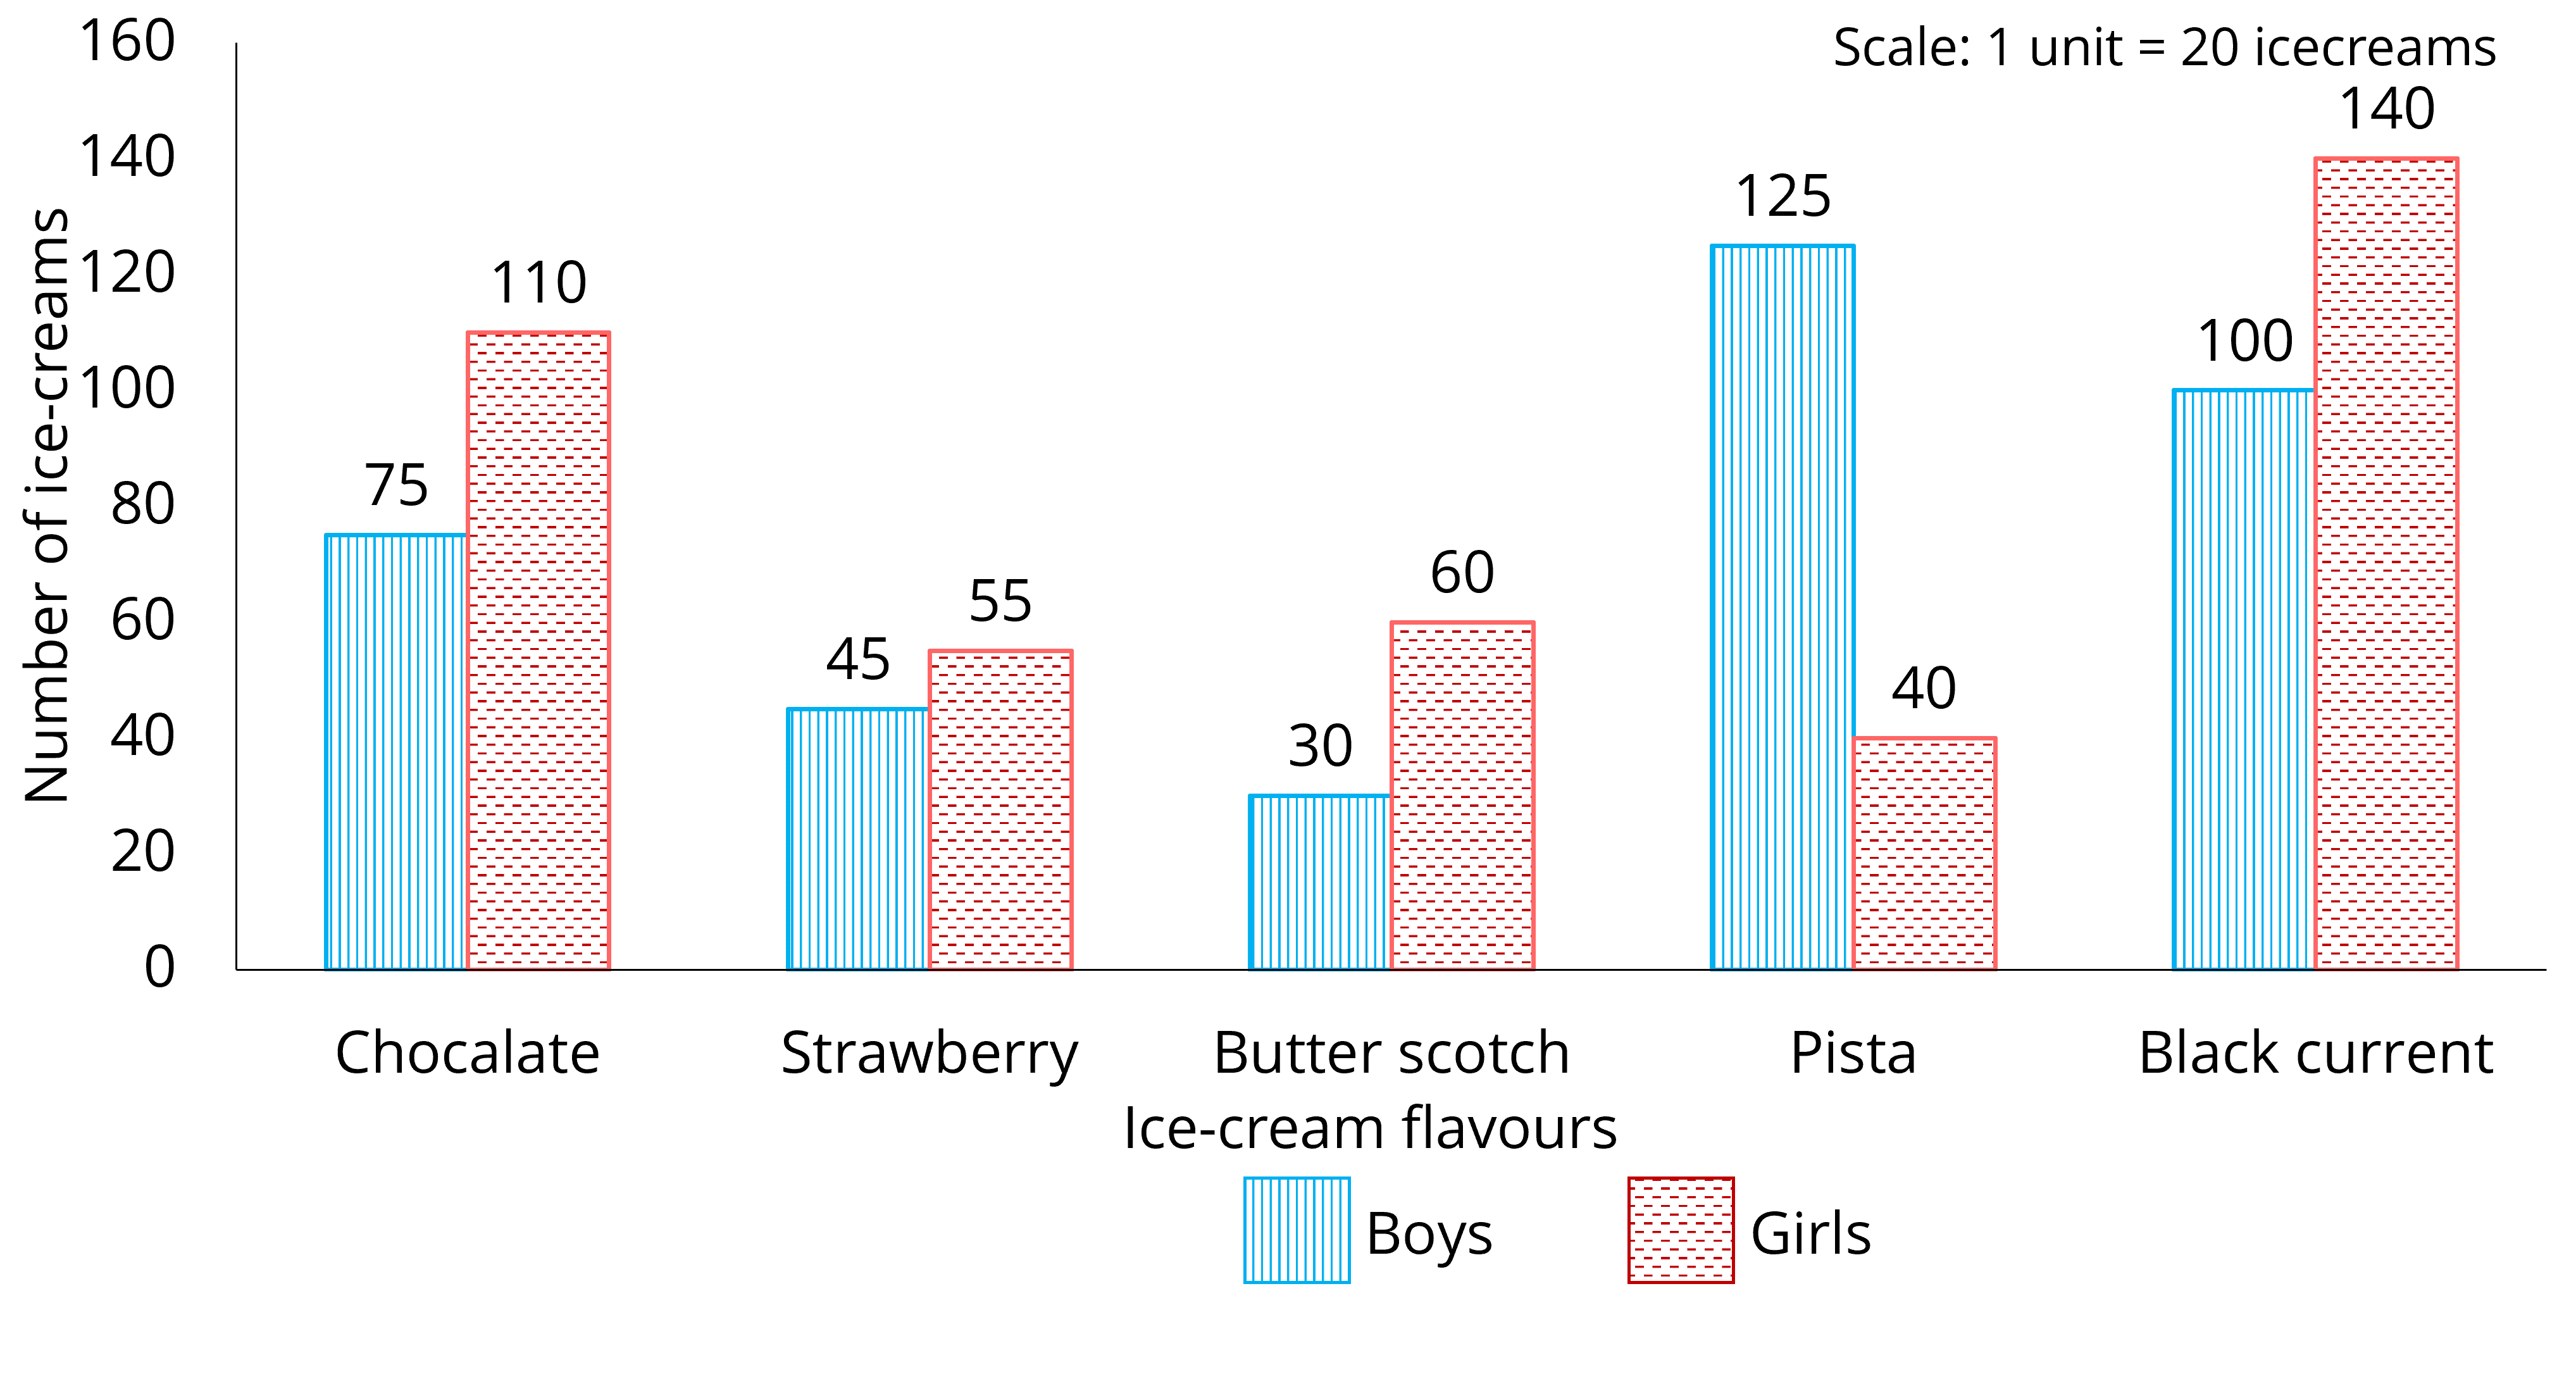
\includegraphics[height = 4cm, width =8cm]{C7M17 - DT - Q5.png}} \\
  i. Identify the flavour that is liked by the maximum number of girls.\\
  ii. Identify the flavour that is liked by the minimum number of boys.},
  optionA={i. Pista, ii. Pista},
  optionB={i. Black current, ii. Butter scotch},
  optionC={i. Pista, ii. Black current},
  optionD={i. Chocolate, ii. Strawberry},
  correctoption={B},
}

\begin{minipage}{\linewidth}
\hspace{1cm}
\centering
\tiny
\renewcommand{\arraystretch}{1.25}
\begin{tabular}{|M{1.2cm}|M{0.8cm}|M{0.8cm}|M{0.8cm}|M{0.8cm}|M{0.8cm}|}
\hline
Option & A (\ding{55}) & \cellcolor{cellgreen} B (\ding{51}) & C (\ding{55}) & D (\ding{55}) & E \\ 
\hline
7 A & \highno{6\%} & \highgreen{81\%} & \highno{13\%} & \highno{0\%} & \highno{0\%} \\ 
 \hline 
7 B & \highno{0\%} & \highgreen{86\%} & \highno{7\%} & \highno{7\%} & \highno{0\%} \\ \hline
\end{tabular}
\end{minipage}

\end{frame}
% \input{4. PPT/My Answer/Math/C7/117_C7M - Q56}


\begin{frame}[shrink=0.1,label=QPC7QC7M07 - DT - Q10]{Q16 [4. Simple Equations]}
\vspace{-0.2cm}
\mcqtextbottomOneFour{
  questionnumber={16}, 
  questionTag={C7M07 – DT – Q10}, 
  questiontext={The difference between 5 times a number and 5 is 40. Determine the number. },
  optionA={5},
  optionB={7},
  optionC={9},
  optionD={15},
  correctoption={C},
}

\begin{minipage}{\linewidth}
\hspace{1cm}
\centering
\tiny
\renewcommand{\arraystretch}{1.25}
\begin{tabular}{|M{1.2cm}|M{0.8cm}|M{0.8cm}|M{0.8cm}|M{0.8cm}|M{0.8cm}|}
\hline
Option & A (\ding{55}) & B (\ding{55}) & \cellcolor{cellgreen} C (\ding{51}) & D (\ding{55}) & E \\ 
\hline
7 A & \highno{0\%} & \highno{13\%} & \highno{50\%} & \highno{19\%} & \highno{19\%} \\ 
 \hline 
7 B & \highno{14\%} & \highno{21\%} & \highred{36\%} & \highno{29\%} & \highno{0\%} \\ \hline
\end{tabular}
\end{minipage}

\end{frame}
% \input{4. PPT/My Answer/Math/C7/117_C7M - Q16}


\begin{frame}[shrink=0.1,label=QPC7QC7M07 - DT - Q8]{Q31 [4. Simple Equations]}
\vspace{-0.2cm}
\mcqimgleftFourOne{
  questionnumber={31}, 
  questionTag={C7M07 – DT – Q8},
  questiontext={To balance both sides of weighing balance, what will be the value of $x$?},
  imgtabletikz = {
 \adjustbox{scale=\scalefactor}{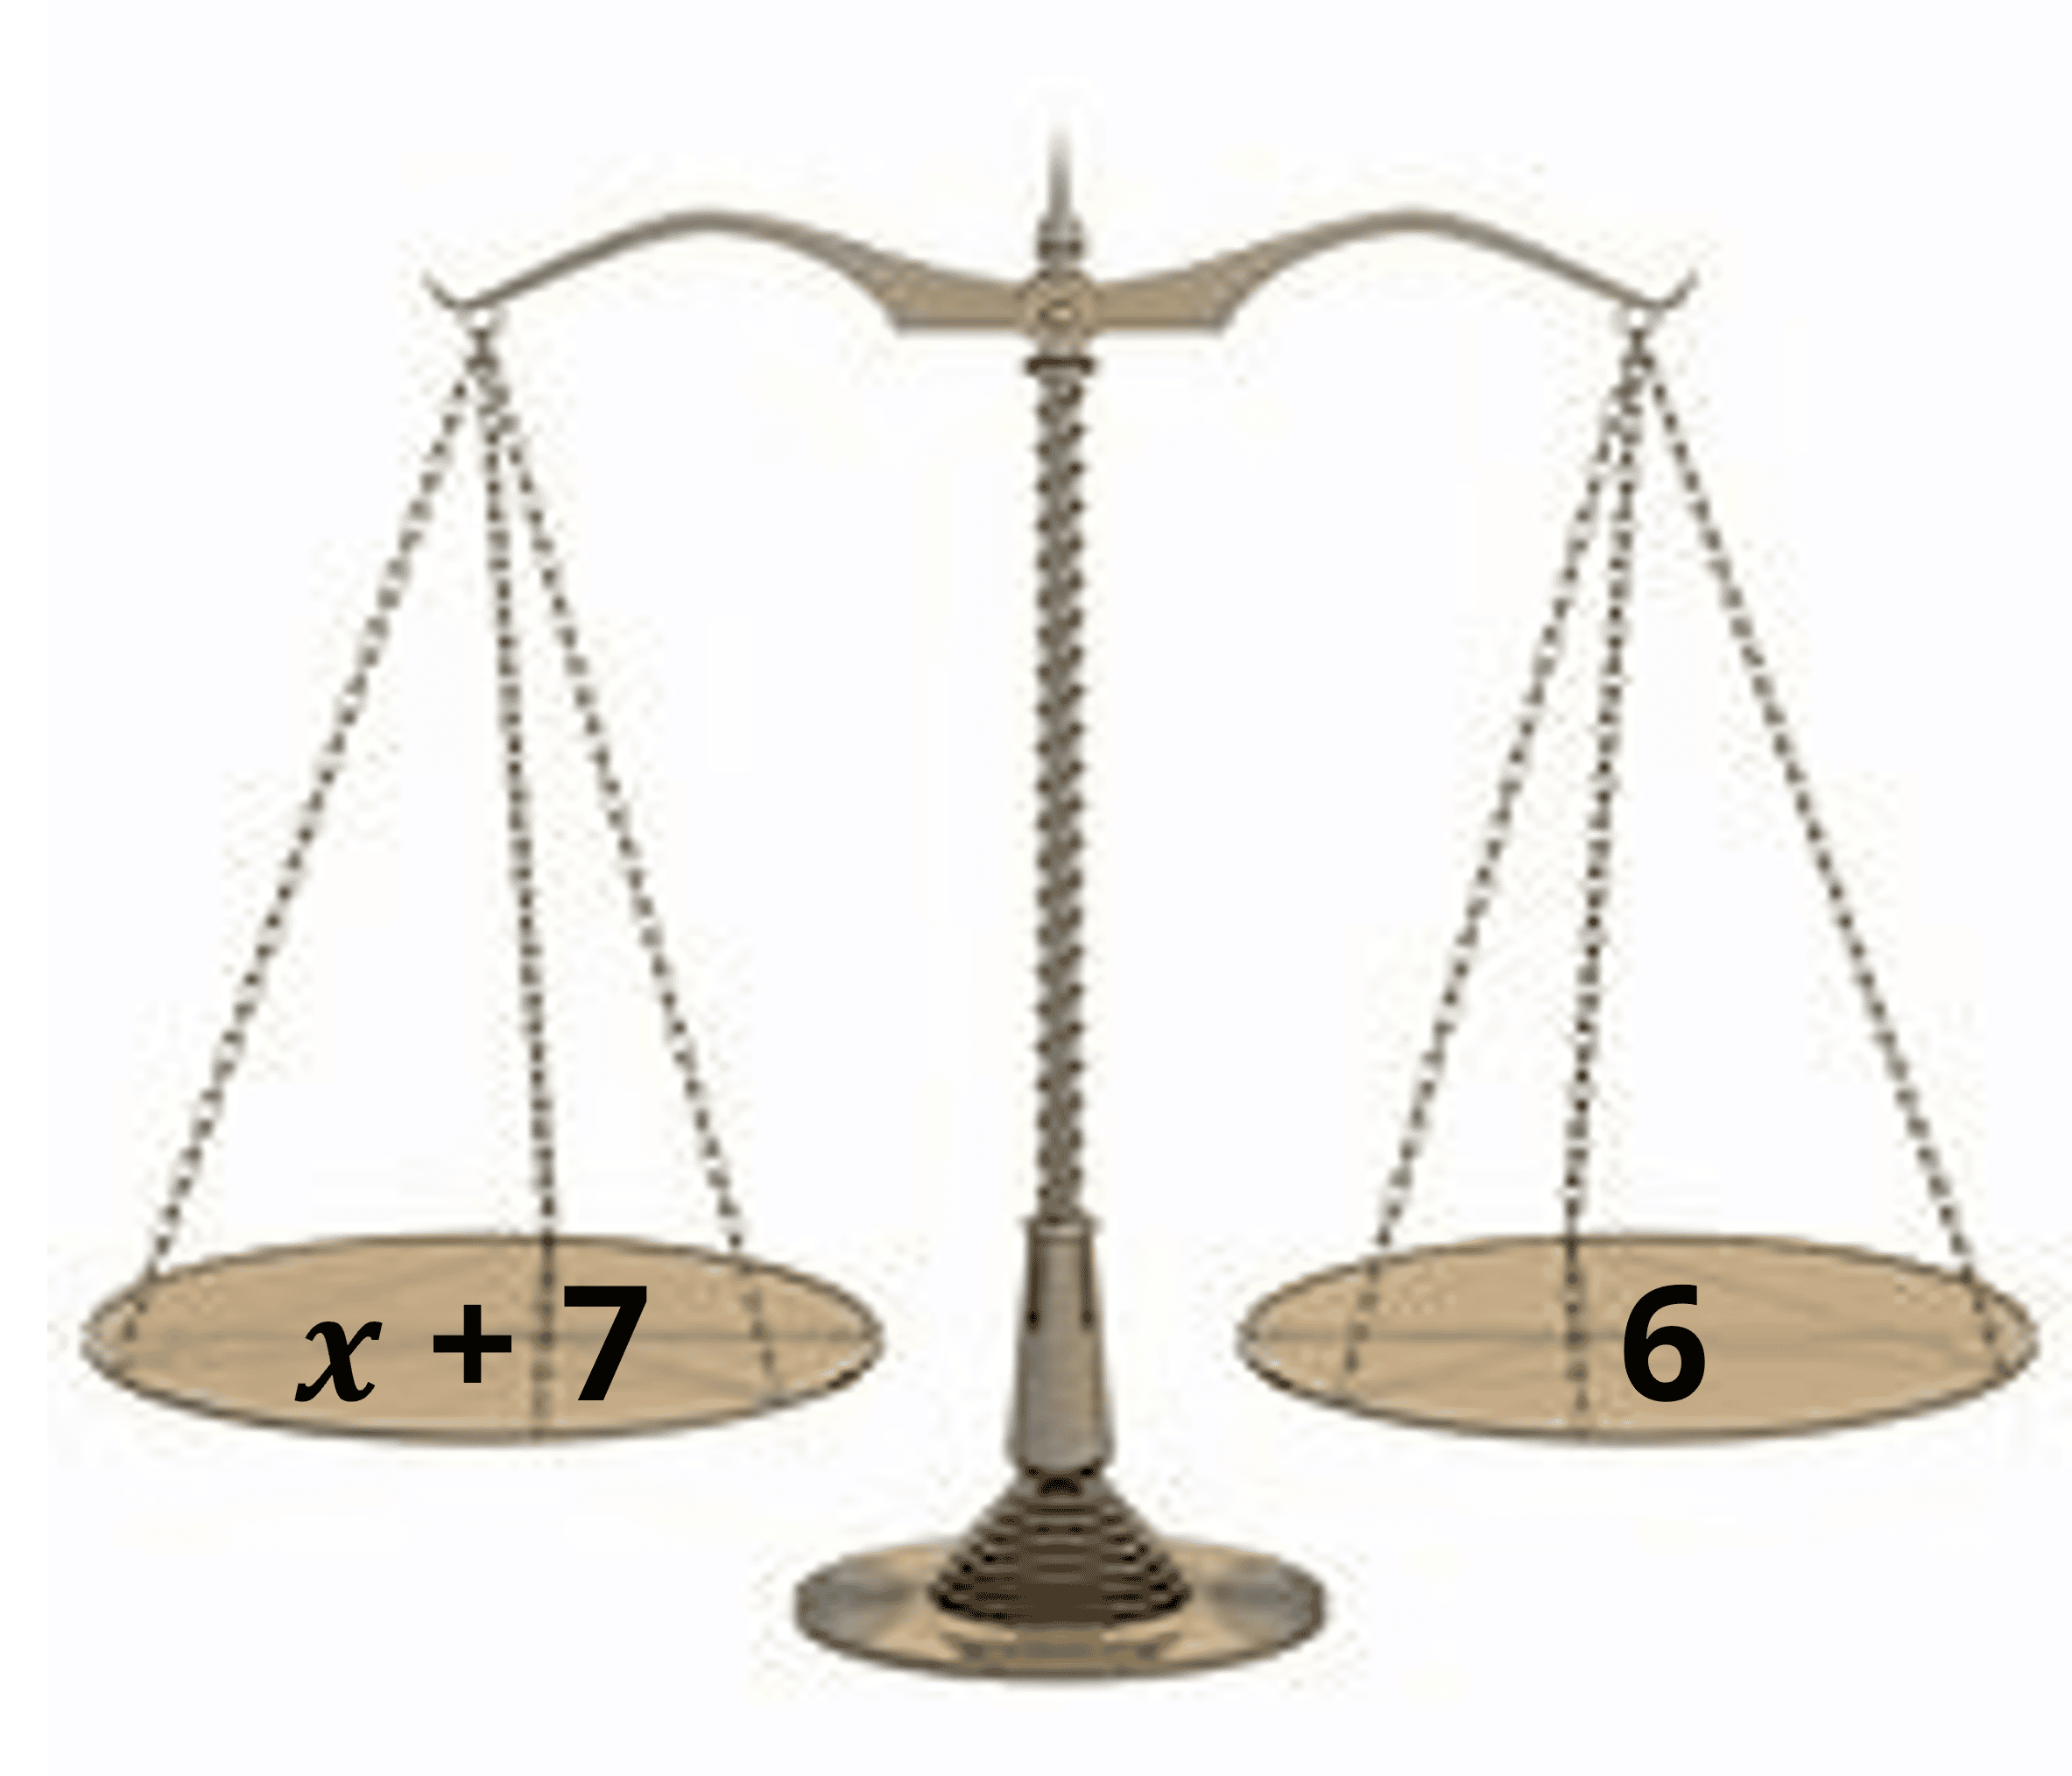
\includegraphics[height=5cm, width = 7cm]{C7M07 - DT - Q8.png}} 
  },
  optionA={13},
  optionB={$-$6},
  optionC={1},
  optionD={$-$1},
  correctoption={D},
  leftmini={0.5},
  rightmini={0.4},}


\begin{minipage}{\linewidth}
\hspace{1cm}
\centering
\tiny
\renewcommand{\arraystretch}{1.25}
\begin{tabular}{|M{1.2cm}|M{0.8cm}|M{0.8cm}|M{0.8cm}|M{0.8cm}|M{0.8cm}|}
\hline
Option & A (\ding{55}) & B (\ding{55}) & C (\ding{55}) & \cellcolor{cellgreen} D (\ding{51}) & E \\ 
\hline
7 A & \highno{19\%} & \highno{0\%} & \highno{19\%} & \highno{63\%} & \highno{0\%} \\ 
 \hline 
7 B & \highno{14\%} & \highno{0\%} & \highno{29\%} & \highno{50\%} & \highno{7\%} \\ \hline
\end{tabular}
\end{minipage}

\end{frame}
% \input{4. PPT/My Answer/Math/C7/117_C7M - Q31}


\begin{frame}[shrink=0.1,label=QPC7QC7M07 - DT - Q4]{Q41 [4. Simple Equations]}
\vspace{-0.2cm}
\mcqtextbottomOneFour{
  questionnumber={41}, 
  questionTag={C7M07 – DT – Q4}, 
  questiontext={Frame the expression for the given statement.\\ \hspace{2.75cm} $c$ added to $v$ is divided by $f$},
  optionA={$\dfrac{vc}{f}$},
  optionB={c + $\dfrac{v}{f}$},
  optionC={$\dfrac{v + c}{f}$},
  optionD={$\dfrac{c + v}{2}$},
  correctoption={C},
}

\begin{minipage}{\linewidth}
\hspace{1cm}
\centering
\tiny
\renewcommand{\arraystretch}{1.25}
\begin{tabular}{|M{1.2cm}|M{0.8cm}|M{0.8cm}|M{0.8cm}|M{0.8cm}|M{0.8cm}|}
\hline
Option & A (\ding{55}) & B (\ding{55}) & \cellcolor{cellgreen} C (\ding{51}) & D (\ding{55}) & E \\ 
\hline
7 A & \highno{0\%} & \highno{50\%} & \highno{44\%} & \highno{6\%} & \highno{0\%} \\ 
 \hline 
7 B & \highno{0\%} & \highno{29\%} & \highno{57\%} & \highno{14\%} & \highno{0\%} \\ \hline
\end{tabular}
\end{minipage}

\end{frame}
% \input{4. PPT/My Answer/Math/C7/117_C7M - Q41}


\begin{frame}[shrink=0.1,label=QPC7QC7M07 - DT - Q5]{Q55 [4. Simple Equations]}
\vspace{-0.2cm}
\mcqtextbottomOneFour{
  questionnumber={55}, 
  questionTag={C7M07 – DT – Q5}, 
  questiontext={Identify the equation.},
  optionA={a + 1 $-$ 2 },
  optionB={$v + 1 > 7 $},
  optionC={$b = 2y$},
  optionD={None of these},
  correctoption={C},
}

\begin{minipage}{\linewidth}
\hspace{1cm}
\centering
\tiny
\renewcommand{\arraystretch}{1.25}
\begin{tabular}{|M{1.2cm}|M{0.8cm}|M{0.8cm}|M{0.8cm}|M{0.8cm}|M{0.8cm}|}
\hline
Option & A (\ding{55}) & B (\ding{55}) & \cellcolor{cellgreen} C (\ding{51}) & D (\ding{55}) & E \\ 
\hline
7 A & \highno{0\%} & \highno{0\%} & \highred{38\%} & \highno{56\%} & \highno{6\%} \\ 
 \hline 
7 B & \highno{7\%} & \highno{0\%} & \highred{36\%} & \highno{43\%} & \highno{14\%} \\ \hline
\end{tabular}
\end{minipage}

\end{frame}
% \input{4. PPT/My Answer/Math/C7/117_C7M - Q55}


\begin{frame}[shrink=0.1,label=QPC7QC7M10 - DT - Q6]{Q30 [5. Lines and Angles]}
\vspace{-0.2cm}
\mcqtextbottomOneFour{
  questionnumber={30}, 
  questionTag={C7M10 – DT – Q6}, 
  questiontext={Find the complementary angle for 90$^\circ$.},
  optionA={180$^\circ$ },
  optionB={90$^\circ$},
  optionC={0$^\circ$},
  optionD={360$^\circ$},
  correctoption={C},
}

\begin{minipage}{\linewidth}
\hspace{1cm}
\centering
\tiny
\renewcommand{\arraystretch}{1.25}
\begin{tabular}{|M{1.2cm}|M{0.8cm}|M{0.8cm}|M{0.8cm}|M{0.8cm}|M{0.8cm}|}
\hline
Option & A (\ding{55}) & B (\ding{55}) & \cellcolor{cellgreen} C (\ding{51}) & D (\ding{55}) & E \\ 
\hline
7 A & \highno{13\%} & \highno{25\%} & \highno{56\%} & \highno{0\%} & \highno{6\%} \\ 
 \hline 
7 B & \highno{36\%} & \highno{29\%} & \highred{36\%} & \highno{0\%} & \highno{0\%} \\ \hline
\end{tabular}
\end{minipage}

\end{frame}
% \input{4. PPT/My Answer/Math/C7/117_C7M - Q30}


\begin{frame}[shrink=0.1,label=QPC7QC7M10 - DT - Q2]{Q52 [5. Lines and Angles]}
\vspace{-0.2cm}
\mcqtextbottomOneFour{
  questionnumber={52}, 
  questionTag={C7M10 – DT – Q2}, 
  questiontext={The angle that lies between 0$^\circ$ and 90$^\circ$ is called a/an \rule{30pt}{0.5pt} angle.},
  optionA={Acute },
  optionB={Right },
  optionC={Obtuse},
  optionD={Zero},
  correctoption={A},
}

\begin{minipage}{\linewidth}
\hspace{1cm}
\centering
\tiny
\renewcommand{\arraystretch}{1.25}
\begin{tabular}{|M{1.2cm}|M{0.8cm}|M{0.8cm}|M{0.8cm}|M{0.8cm}|M{0.8cm}|}
\hline
Option & \cellcolor{cellgreen} A (\ding{51}) & B (\ding{55}) & C (\ding{55}) & D (\ding{55}) & E \\ 
\hline
7 A & \highred{38\%} & \highno{50\%} & \highno{6\%} & \highno{6\%} & \highno{0\%} \\ 
 \hline 
7 B & \highno{50\%} & \highno{36\%} & \highno{14\%} & \highno{0\%} & \highno{0\%} \\ \hline
\end{tabular}
\end{minipage}

\end{frame}
% \input{4. PPT/My Answer/Math/C7/117_C7M - Q52}


\begin{frame}[shrink=0.1,label=QPC7QC7M10 - DT - Q9]{Q54 [5. Lines and Angles]}
\vspace{-0.2cm}
\mcqimgleftFourOne{
questionnumber={54}, 
  questionTag={C7M10 – DT – Q9},
  questiontext={Find the relationship between $\angle$2 and $\angle$6.},
  imgtabletikz = { 
\tikzset{every picture/.style={line width=0.75pt,scale=\scalefactor}}
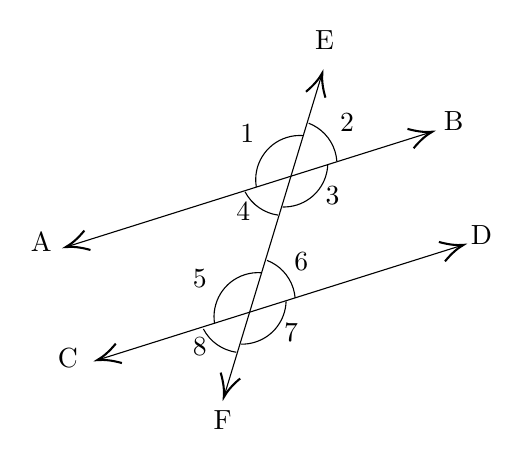
\begin{tikzpicture}[x=0.75pt,y=0.75pt,yscale=-1,xscale=1]
\draw    (207,114.84) -- (379.72,60.48) ;
\draw [shift={(381.63,59.88)}, rotate = 162.53] [color={rgb, 255:red, 0; green, 0; blue, 0 }  ][line width=0.75]    (10.93,-4.9) .. controls (6.95,-2.3) and (3.31,-0.67) .. (0,0) .. controls (3.31,0.67) and (6.95,2.3) .. (10.93,4.9)   ;
\draw [shift={(205.09,115.44)}, rotate = 342.53] [color={rgb, 255:red, 0; green, 0; blue, 0 }  ][line width=0.75]    (10.93,-4.9) .. controls (6.95,-2.3) and (3.31,-0.67) .. (0,0) .. controls (3.31,0.67) and (6.95,2.3) .. (10.93,4.9)   ;
\draw    (281.8,185.88) -- (328.1,33.47) ;
\draw [shift={(328.68,31.56)}, rotate = 106.9] [color={rgb, 255:red, 0; green, 0; blue, 0 }  ][line width=0.75]    (10.93,-4.9) .. controls (6.95,-2.3) and (3.31,-0.67) .. (0,0) .. controls (3.31,0.67) and (6.95,2.3) .. (10.93,4.9)   ;
\draw [shift={(281.22,187.8)}, rotate = 286.9] [color={rgb, 255:red, 0; green, 0; blue, 0 }  ][line width=0.75]    (10.93,-4.9) .. controls (6.95,-2.3) and (3.31,-0.67) .. (0,0) .. controls (3.31,0.67) and (6.95,2.3) .. (10.93,4.9)   ;
\draw    (222.13,169.32) -- (394.85,114.96) ;
\draw [shift={(396.75,114.36)}, rotate = 162.53] [color={rgb, 255:red, 0; green, 0; blue, 0 }  ][line width=0.75]    (10.93,-4.9) .. controls (6.95,-2.3) and (3.31,-0.67) .. (0,0) .. controls (3.31,0.67) and (6.95,2.3) .. (10.93,4.9)   ;
\draw [shift={(220.22,169.92)}, rotate = 342.53] [color={rgb, 255:red, 0; green, 0; blue, 0 }  ][line width=0.75]    (10.93,-4.9) .. controls (6.95,-2.3) and (3.31,-0.67) .. (0,0) .. controls (3.31,0.67) and (6.95,2.3) .. (10.93,4.9)   ;
\draw  [draw opacity=0] (302.05,121.85) .. controls (307.87,124.1) and (312.65,128.88) .. (314.67,135.29) .. controls (315.16,136.86) and (315.46,138.44) .. (315.59,140.02) -- (294.4,141.67) -- cycle ; \draw   (302.05,121.85) .. controls (307.87,124.1) and (312.65,128.88) .. (314.67,135.29) .. controls (315.16,136.86) and (315.46,138.44) .. (315.59,140.02) ;   
\draw  [draw opacity=0] (311.23,141.63) .. controls (310.95,150.41) and (305.21,158.44) .. (296.36,161.23) .. controls (294.08,161.95) and (291.76,162.26) .. (289.49,162.21) -- (289.99,140.96) -- cycle ; \draw   (311.23,141.63) .. controls (310.95,150.41) and (305.21,158.44) .. (296.36,161.23) .. controls (294.08,161.95) and (291.76,162.26) .. (289.49,162.21) ;  
\draw  [draw opacity=0] (276.79,152.46) .. controls (275.09,142.18) and (281.16,131.95) .. (291.38,128.73) .. controls (294,127.91) and (296.65,127.62) .. (299.23,127.8) -- (297.76,149) -- cycle ; \draw   (276.79,152.46) .. controls (275.09,142.18) and (281.16,131.95) .. (291.38,128.73) .. controls (294,127.91) and (296.65,127.62) .. (299.23,127.8) ;  
\draw  [draw opacity=0] (287.21,166.11) .. controls (280.57,165.15) and (274.6,161.06) .. (271.4,154.92) -- (290.23,145.08) -- cycle ; \draw   (287.21,166.11) .. controls (280.57,165.15) and (274.6,161.06) .. (271.4,154.92) ;  
\draw  [draw opacity=0] (322.14,55.77) .. controls (327.96,58.02) and (332.74,62.8) .. (334.76,69.21) .. controls (335.25,70.78) and (335.55,72.36) .. (335.68,73.94) -- (314.49,75.59) -- cycle ; \draw   (322.14,55.77) .. controls (327.96,58.02) and (332.74,62.8) .. (334.76,69.21) .. controls (335.25,70.78) and (335.55,72.36) .. (335.68,73.94) ;   
\draw  [draw opacity=0] (331.32,75.55) .. controls (331.04,84.33) and (325.3,92.36) .. (316.45,95.15) .. controls (314.17,95.87) and (311.85,96.18) .. (309.58,96.13) -- (310.08,74.88) -- cycle ; \draw   (331.32,75.55) .. controls (331.04,84.33) and (325.3,92.36) .. (316.45,95.15) .. controls (314.17,95.87) and (311.85,96.18) .. (309.58,96.13) ;  
\draw  [draw opacity=0] (296.88,86.38) .. controls (295.18,76.1) and (301.25,65.87) .. (311.47,62.66) .. controls (314.09,61.83) and (316.74,61.54) .. (319.32,61.72) -- (317.85,82.92) -- cycle ; \draw   (296.88,86.38) .. controls (295.18,76.1) and (301.25,65.87) .. (311.47,62.66) .. controls (314.09,61.83) and (316.74,61.54) .. (319.32,61.72) ;  
\draw  [draw opacity=0] (307.3,100.03) .. controls (300.66,99.07) and (294.69,94.98) .. (291.49,88.84) -- (310.32,79) -- cycle ; \draw   (307.3,100.03) .. controls (300.66,99.07) and (294.69,94.98) .. (291.49,88.84) ;  
\draw (288,55) node [anchor=north west][inner sep=0.75pt]   [align=left] {1};
\draw (336,50) node [anchor=north west][inner sep=0.75pt]   [align=left] {2};
\draw (329,85) node [anchor=north west][inner sep=0.75pt]   [align=left] {3};
\draw (286,93) node [anchor=north west][inner sep=0.75pt]   [align=left] {4};
\draw (399,104) node [anchor=north west][inner sep=0.75pt]   [align=left] {D};
\draw (200,163) node [anchor=north west][inner sep=0.75pt]   [align=left] {C};
\draw (386,49) node [anchor=north west][inner sep=0.75pt]   [align=left] {B};
\draw (187,107) node [anchor=north west][inner sep=0.75pt]   [align=left] {A};
\draw (275,193) node [anchor=north west][inner sep=0.75pt]   [align=left] {F};
\draw (324,10) node [anchor=north west][inner sep=0.75pt]   [align=left] {E};
\draw (265,158) node [anchor=north west][inner sep=0.75pt]   [align=left] {8};
\draw (309,151) node [anchor=north west][inner sep=0.75pt]   [align=left] {7};
\draw (314,117) node [anchor=north west][inner sep=0.75pt]   [align=left] {6};
\draw (265,125) node [anchor=north west][inner sep=0.75pt]   [align=left] {5};
\end{tikzpicture} },
  optionA={Linear pair},
  optionB={Co-interior},
  optionC={Corresponding angle},
  optionD={Vertically opposite},
  correctoption={C},
  leftmini={0.5},
  rightmini={0.4},}

\begin{minipage}{\linewidth}
\hspace{1cm}
\centering
\tiny
\renewcommand{\arraystretch}{1.25}
\begin{tabular}{|M{1.2cm}|M{0.8cm}|M{0.8cm}|M{0.8cm}|M{0.8cm}|M{0.8cm}|}
\hline
Option & A (\ding{55}) & B (\ding{55}) & \cellcolor{cellgreen} C (\ding{51}) & D (\ding{55}) & E \\ 
\hline
7 A & \highno{6\%} & \highno{0\%} & \highgreen{94\%} & \highno{0\%} & \highno{0\%} \\ 
 \hline 
7 B & \highno{14\%} & \highno{0\%} & \highgreen{86\%} & \highno{0\%} & \highno{0\%} \\ \hline
\end{tabular}
\end{minipage}

\end{frame}
% \input{4. PPT/My Answer/Math/C7/117_C7M - Q54}


\begin{frame}[shrink=0.1,label=QPC7QC7M11 - DT - Q6]{Q14 [6. The Triangles and Its Properties]}
\vspace{-0.2cm}
\mcqtextbottomOneFour{
  questionnumber={14}, 
  questionTag={C7M11 - DT - Q6}, 
  questiontext={If two angles of a triangle are 46$^\circ$ and 55$^\circ$, what is the third angle?},
  optionA={180$^\circ$},
  optionB={90$^\circ$},
  optionC={79$^\circ$},
  optionD={101$^\circ$},
  correctoption={C},
}

\begin{minipage}{\linewidth}
\hspace{1cm}
\centering
\tiny
\renewcommand{\arraystretch}{1.25}
\begin{tabular}{|M{1.2cm}|M{0.8cm}|M{0.8cm}|M{0.8cm}|M{0.8cm}|M{0.8cm}|}
\hline
Option & A (\ding{55}) & B (\ding{55}) & \cellcolor{cellgreen} C (\ding{51}) & D (\ding{55}) & E \\ 
\hline
7 A & \highno{0\%} & \highno{6\%} & \highno{44\%} & \highno{50\%} & \highno{0\%} \\ 
 \hline 
7 B & \highno{7\%} & \highno{14\%} & \highred{36\%} & \highno{43\%} & \highno{0\%} \\ \hline
\end{tabular}
\end{minipage}

\end{frame}
% \input{4. PPT/My Answer/Math/C7/117_C7M - Q14}


\begin{frame}[shrink=0.1,label=QPC7QC7M11 - DT - Q8]{Q23 [6. The Triangles and Its Properties]}
\vspace{-0.2cm}
\mcqimgleftFourOne{
  questionnumber={23}, 
  questionTag={C7M11 - DT - Q8},
  questiontext={Find the side length AB.},
  imgtabletikz = {
\tikzset{every picture/.style={line width=0.75pt,scale=\scalefactor}} 
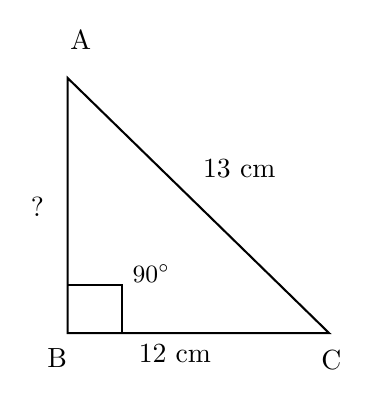
\begin{tikzpicture}[x=0.75pt,y=0.75pt,yscale=-1,xscale=1]
\draw  [line width=0.75]  (100,104) -- (226,226.92) -- (100,226.92) -- cycle ;
\draw  [line width=0.75]  (100,203.85) -- (126,203.85) -- (126,226.92) ;
\draw (100,80) node [anchor=north west][inner sep=0.75pt]   [align=left] {A};
\draw (89,233) node [anchor=north west][inner sep=0.75pt]   [align=left] {B};
\draw (221,234) node [anchor=north west][inner sep=0.75pt]   [align=left] {C};
\draw (133,231) node [anchor=north west][inner sep=0.75pt]   [align=left] {12 cm};
\draw (164,142) node [anchor=north west][inner sep=0.75pt]   [align=left] {13 cm};
\draw (81,160) node [anchor=north west][inner sep=0.75pt]   [align=left] {?};
\draw (130,192.4) node [anchor=north west][inner sep=0.75pt]  [font=\small]  {90$^\circ$};
\end{tikzpicture} },
  optionA={5 cm},
  optionB={10 cm},
  optionC={3 cm},
  optionD={25 cm},
  correctoption={A},
  leftmini={0.5},
  rightmini={0.4},
}

\begin{minipage}{\linewidth}
\hspace{1cm}
\centering
\tiny
\renewcommand{\arraystretch}{1.25}
\begin{tabular}{|M{1.2cm}|M{0.8cm}|M{0.8cm}|M{0.8cm}|M{0.8cm}|M{0.8cm}|}
\hline
Option & \cellcolor{cellgreen} A (\ding{51}) & B (\ding{55}) & C (\ding{55}) & D (\ding{55}) & E \\ 
\hline
7 A & \highred{25\%} & \highno{19\%} & \highno{0\%} & \highno{50\%} & \highno{6\%} \\ 
 \hline 
7 B & \highred{36\%} & \highno{0\%} & \highno{0\%} & \highno{57\%} & \highno{7\%} \\ \hline
\end{tabular}
\end{minipage}

\end{frame}
% \input{4. PPT/My Answer/Math/C7/117_C7M - Q23}


\begin{frame}[shrink=0.1,label=QPC7QC7M11 - DT - Q2]{Q26 [6. The Triangles and Its Properties]}
\vspace{-0.2cm}
\mcqimgleftFourOne{
questionnumber={26}, 
  questionTag={C7M11 – DT – Q2},
  questiontext={In the triangle $\Delta$ABE, D is the midpoint of BE, then AD is a \rule{30pt}{0.5pt}.},
 imgtabletikz = {
\tikzset{every picture/.style={line width=0.75pt,scale=\scalefactor}}      
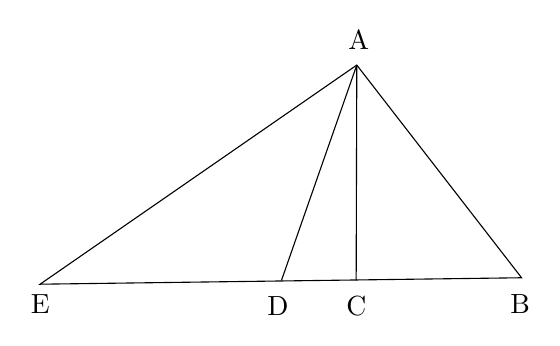
\begin{tikzpicture}[x=0.75pt,y=0.75pt,yscale=-1,xscale=1]
\draw   (228.3,22.75) -- (307.69,125.22) -- (75.71,128.33) -- cycle ;
\draw    (228.3,22.75) -- (228,126.52) ;
\draw    (228.3,22.75) -- (192,126.52) ;
\draw (223,5) node [anchor=north west][inner sep=0.75pt]   [align=left] {A};
\draw (301,132) node [anchor=north west][inner sep=0.75pt]   [align=left] {B};
\draw (222,133) node [anchor=north west][inner sep=0.75pt]   [align=left] {C};
\draw (184,133) node [anchor=north west][inner sep=0.75pt]   [align=left] {D};
\draw (70,132) node [anchor=north west][inner sep=0.75pt]   [align=left] {E};
\end{tikzpicture} },
  optionA={Median },
  optionB={Altitude},
  optionC={Height},
  optionD={Base},
  correctoption={A},
  leftmini={0.5},
  rightmini={0.4},}


\begin{minipage}{\linewidth}
\hspace{1cm}
\centering
\tiny
\renewcommand{\arraystretch}{1.25}
\begin{tabular}{|M{1.2cm}|M{0.8cm}|M{0.8cm}|M{0.8cm}|M{0.8cm}|M{0.8cm}|}
\hline
Option & \cellcolor{cellgreen} A (\ding{51}) & B (\ding{55}) & C (\ding{55}) & D (\ding{55}) & E \\ 
\hline
7 A & \highno{50\%} & \highno{31\%} & \highno{13\%} & \highno{6\%} & \highno{0\%} \\ 
 \hline 
7 B & \highno{43\%} & \highno{50\%} & \highno{0\%} & \highno{7\%} & \highno{0\%} \\ \hline
\end{tabular}
\end{minipage}

\end{frame}
% \input{4. PPT/My Answer/Math/C7/117_C7M - Q26}


\begin{frame}[shrink=0.1,label=QPC7QC7M11 - DT - Q3]{Q46 [6. The Triangles and Its Properties]}
\vspace{-0.2cm}
\mcqimgleftFourOne{
 questionnumber={46}, 
  questionTag={C7M11 – DT – Q3},
  questiontext={Match the following.},
  imgtabletikz = {
\centering
\renewcommand{\arraystretch}{1.25}
    \begin{tabular}{|p{0.5cm}|p{2.5cm}|p{0.2cm}|p{0.5cm}|p{3.5cm}|}
      \cline{1-5} 
       \multicolumn{2}{|c|}{\textbf{Types of triangle   
 }} & 
      \multirow{5}{*}{} &   
      \multicolumn{2}{c|}{\textbf{Description}} \\
      \cline{1-2}\cline{4-5} i.  & Isosceles triangle
 &   & a. & 3 sides of different length \\
      \cline{1-2}\cline{4-5} ii. & Scalene triangle &   & b. &  3 sides of equal length\\
      \cline{1-2}\cline{4-5} iii.  & Equilateral triangle &   & c. & 2 sides of equal length  \\
 \hline
    \end{tabular}
    },
 optionA={i - c, ii - a, iii - b},
  optionB={i - c, ii - b, iii - a},
  optionC={i - a, ii - b, iii - c},
  optionD={i - a, ii - c, iii - b},
  correctoption={A},
  leftmini={0.6},
  rightmini={0.3},
}
 

\begin{minipage}{\linewidth}
\hspace{1cm}
\centering
\tiny
\renewcommand{\arraystretch}{1.25}
\begin{tabular}{|M{1.2cm}|M{0.8cm}|M{0.8cm}|M{0.8cm}|M{0.8cm}|M{0.8cm}|}
\hline
Option & \cellcolor{cellgreen} A (\ding{51}) & B (\ding{55}) & C (\ding{55}) & D (\ding{55}) & E \\ 
\hline
7 A & \highno{63\%} & \highno{13\%} & \highno{6\%} & \highno{19\%} & \highno{0\%} \\ 
 \hline 
7 B & \highno{50\%} & \highno{14\%} & \highno{14\%} & \highno{7\%} & \highno{14\%} \\ \hline
\end{tabular}
\end{minipage}

\end{frame}
% \input{4. PPT/My Answer/Math/C7/117_C7M - Q46}


\begin{frame}[shrink=0.1,label=QPC7QC7M11 - CT - Q1]{Q59 [6. The Triangles and Its Properties]}
\vspace{-0.2cm}
\mcqtextbottomOneFour{
  questionnumber={59 - Critical Thinking},
  questionTag = {C7M11 - CT - Q1},
  questiontext = {In the given scalene triangle ABC, \\
  \medskip
  \begin{minipage}{0.35\textwidth}  
\tikzset{every picture/.style={line width=0.75pt,scale=\scalefactor}} 
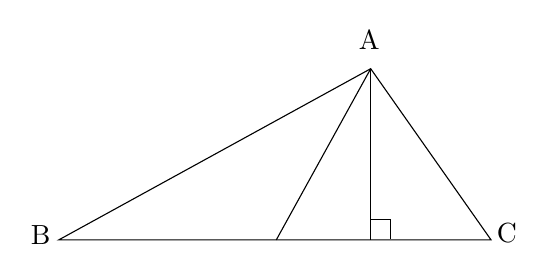
\begin{tikzpicture}[x=0.75pt,y=0.75pt,yscale=-1,xscale=1]
\draw   (390,78.52) -- (448,161.02) -- (239.67,161.02) -- cycle ;
\draw    (390,78.52) -- (390,160.86) ;
\draw    (390,78.52) -- (344.5,161.02) ;
\draw   (390.35,151.29) -- (399.58,151.29) -- (399.58,160.52) ;
\draw (383,59.02) node [anchor=north west][inner sep=0.75pt]   [align=left] {A};
\draw (225,153.02) node [anchor=north west][inner sep=0.75pt]   [align=left] {B};
\draw (449.5,152.02) node [anchor=north west][inner sep=0.75pt]   [align=left] {C};
\end{tikzpicture}
  \end{minipage}
    \begin{minipage}{0.55\textwidth}
      i. 10 cm, 17 cm, and 21 cm are the sides of the triangle. \\
ii. The base of the triangle has larger measurements. \\
iii. The distance between the altitude AX and median AY at the base of the triangle is 4.5 cm.
  \end{minipage}\\ \medskip
What is the height of the triangle in cm? },
  optionA={6},
  optionB={10.5},
  optionC={15},
  optionD={8},
  correctoption = {D},
  }

\begin{minipage}{\linewidth}
\hspace{1cm}
\centering
\tiny
\renewcommand{\arraystretch}{1.25}
\begin{tabular}{|M{1.2cm}|M{0.8cm}|M{0.8cm}|M{0.8cm}|M{0.8cm}|M{0.8cm}|}
\hline
Option & A (\ding{55}) & B (\ding{55}) & C (\ding{55}) & \cellcolor{cellgreen} D (\ding{51}) & E \\ 
\hline
7 A & \highno{6\%} & \highno{63\%} & \highno{19\%} & \highred{0\%} & \highno{13\%} \\ 
 \hline 
7 B & \highno{0\%} & \highno{57\%} & \highno{29\%} & \highred{7\%} & \highno{7\%} \\ \hline
\end{tabular}
\end{minipage}

\end{frame}
% \input{4. PPT/My Answer/Math/C7/117_C7M - Q59 - Critical Thinking}


\begin{frame}[shrink=0.1,label=QPC7QC7M09 - DT - Q1]{Q12 [7. Comparing Quantities]}
\vspace{-0.2cm}
\mcqimgleftFourOne{
  questionnumber={12}, 
  questionTag={C7M09 - DT - Q1},
  questiontext={Find the ratios of father to son and mother to son.},
  imgtabletikz = { 
\tikzset{every picture/.style={line width=0.75pt,scale=\scalefactor}} 
\begin{tikzpicture}[x=0.75pt,y=0.75pt,yscale=-1,xscale=1]
\draw (297,92.55) node  {\adjustbox{scale=\scalefactor}{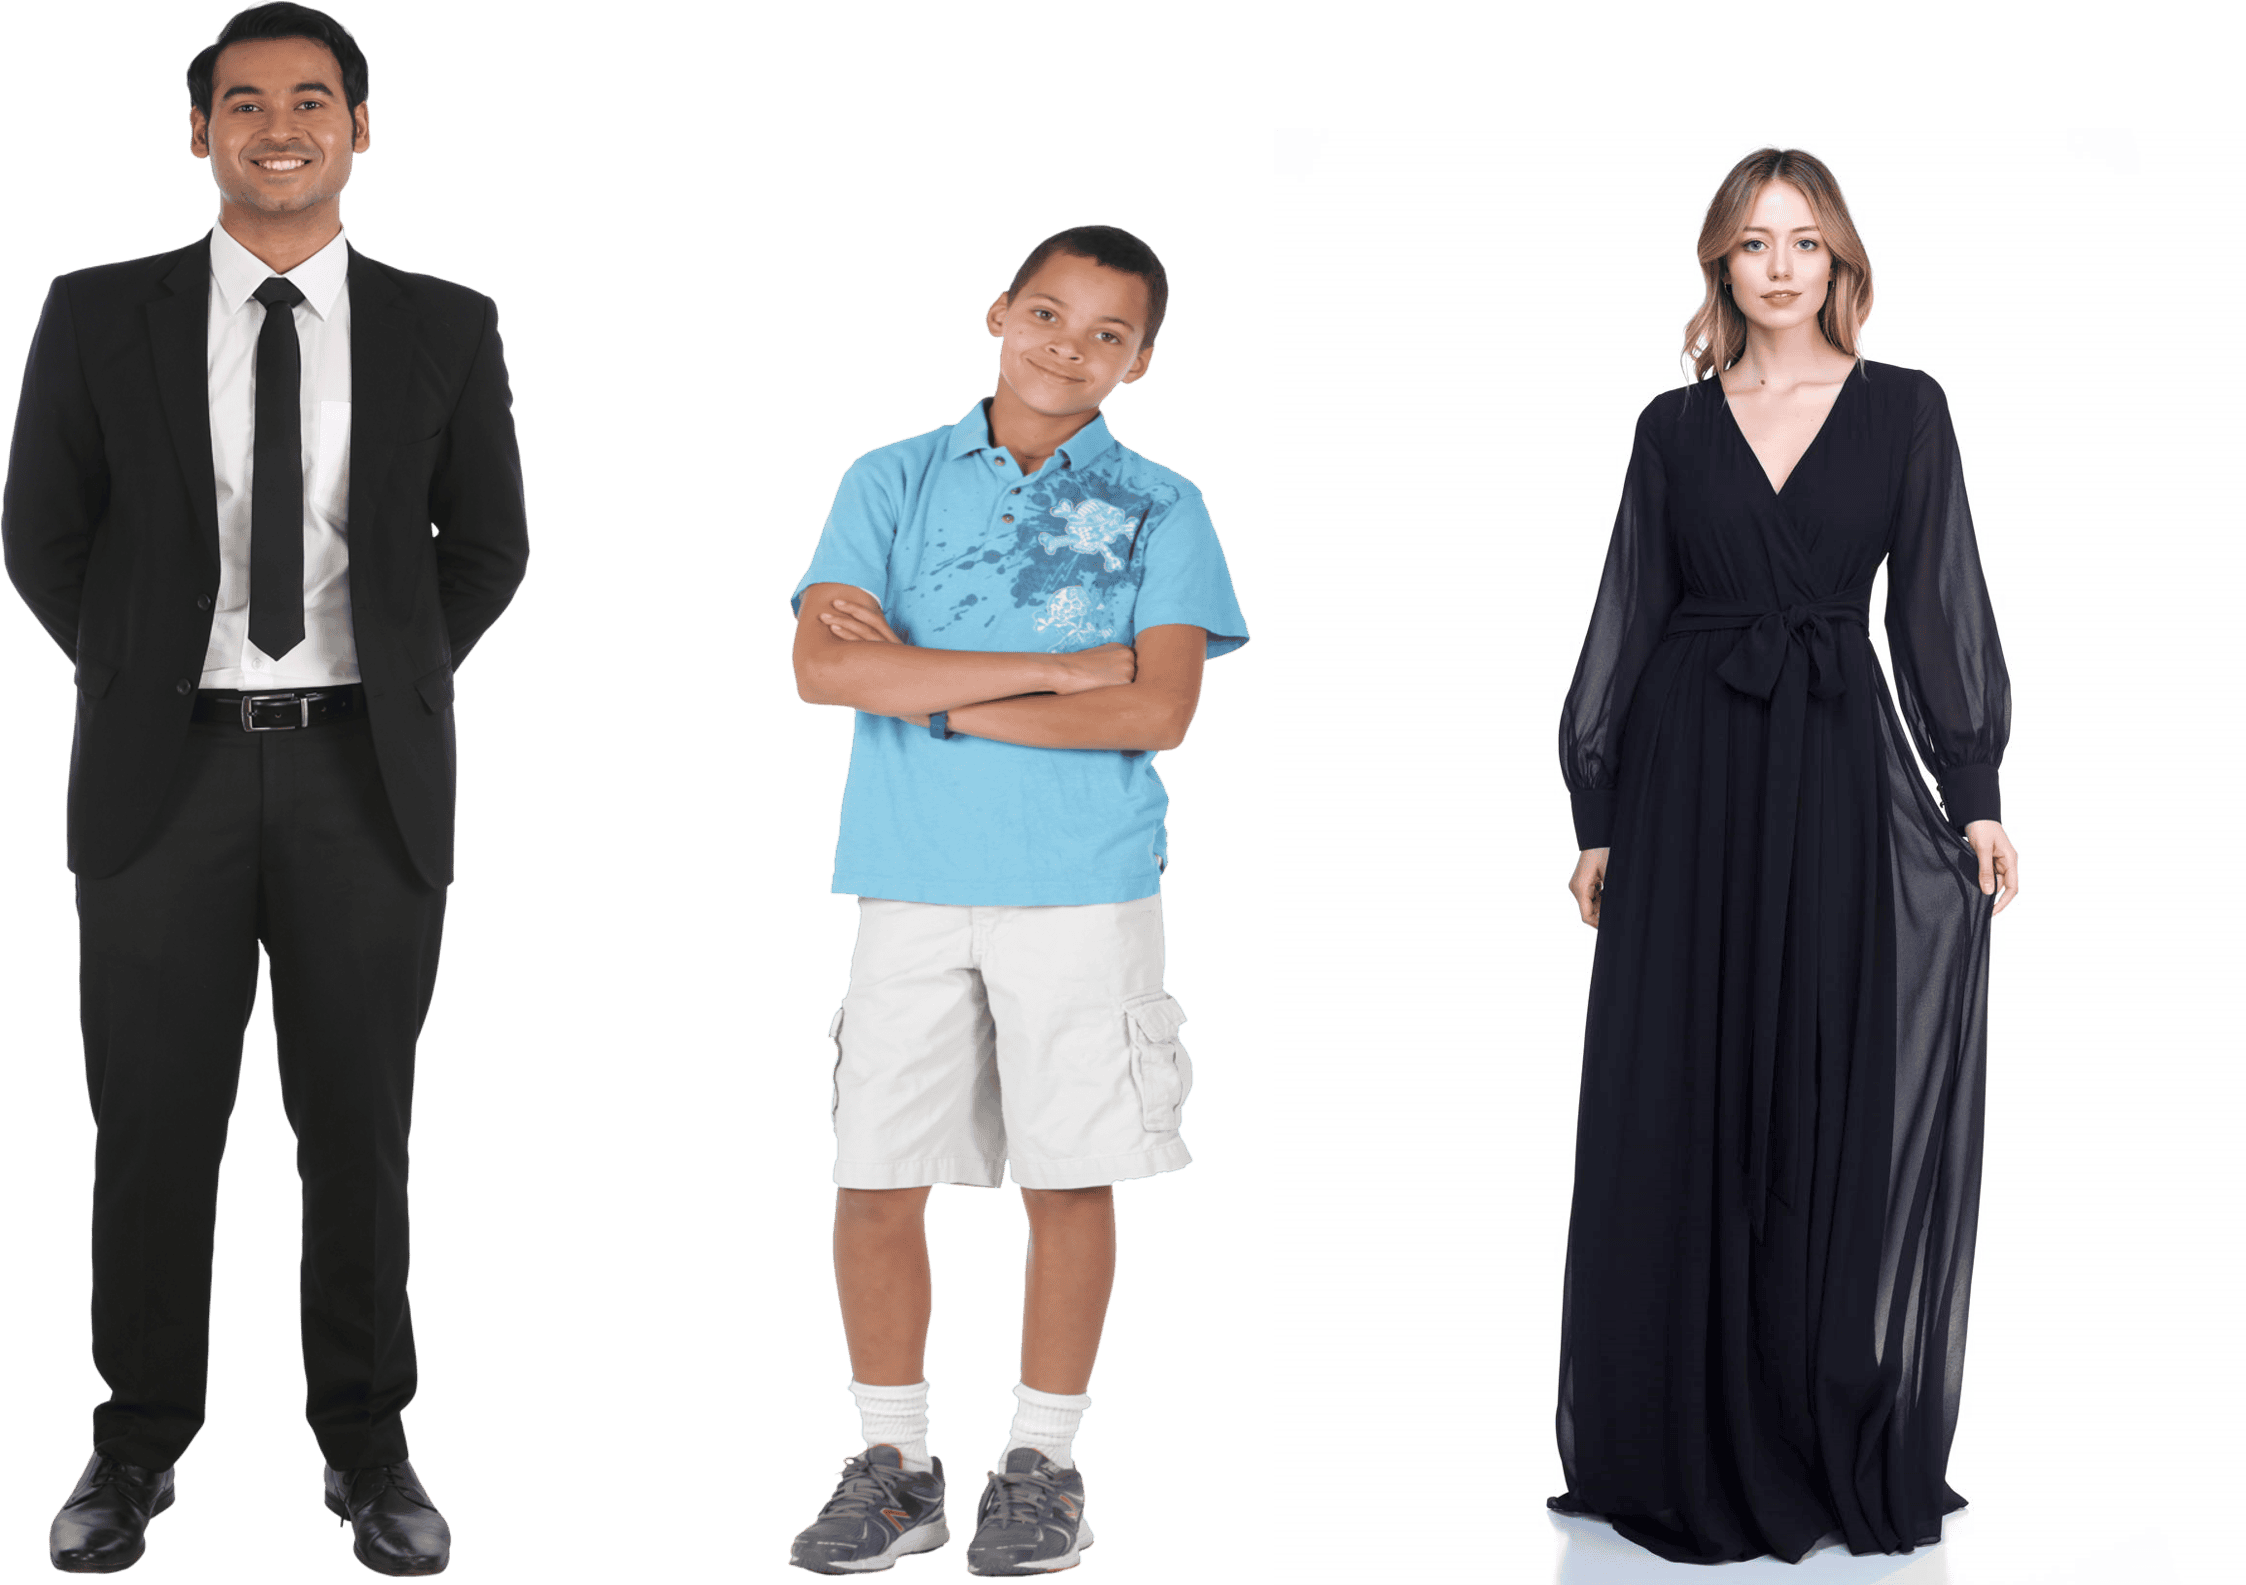
\includegraphics[width=140pt,height=96.83pt]{C7M09 - DT - Q1.png}}};
\draw (195,163) node [anchor=north west][inner sep=0.75pt]   [align=left] {40 years};
\draw (267,163) node [anchor=north west][inner sep=0.75pt]   [align=left] {9 years};
\draw (335,163) node [anchor=north west][inner sep=0.75pt]   [align=left] {35 years};
\end{tikzpicture} },
  optionA={40 : 9, 35 : 9},
  optionB={40 : 9, 9 : 35},
  optionC={35 : 9, 45 : 9},
  optionD={40 : 9, 50 : 9},
  correctoption={A},
  leftmini={0.5},
  rightmini={0.4},
}

\begin{minipage}{\linewidth}
\hspace{1cm}
\centering
\tiny
\renewcommand{\arraystretch}{1.25}
\begin{tabular}{|M{1.2cm}|M{0.8cm}|M{0.8cm}|M{0.8cm}|M{0.8cm}|M{0.8cm}|}
\hline
Option & \cellcolor{cellgreen} A (\ding{51}) & B (\ding{55}) & C (\ding{55}) & D (\ding{55}) & E \\ 
\hline
7 A & \highgreen{81\%} & \highno{13\%} & \highno{6\%} & \highno{0\%} & \highno{0\%} \\ 
 \hline 
7 B & \highgreen{79\%} & \highno{21\%} & \highno{0\%} & \highno{0\%} & \highno{0\%} \\ \hline
\end{tabular}
\end{minipage}

\end{frame}
% \input{4. PPT/My Answer/Math/C7/117_C7M - Q12}


\begin{frame}[shrink=0.1,label=QPC7QC7M09 - DT - Q10]{Q13 [7. Comparing Quantities]}
\vspace{-0.2cm}
\mcqimgleftFourOne{
  questionnumber={13}, 
  questionTag={C7M09 - DT - Q10},
  questiontext={Find the profit earned, if the cost price of the Rubics Cube is Rs. 100.},
  imgtabletikz = { \adjustbox{scale=\scalefactor}{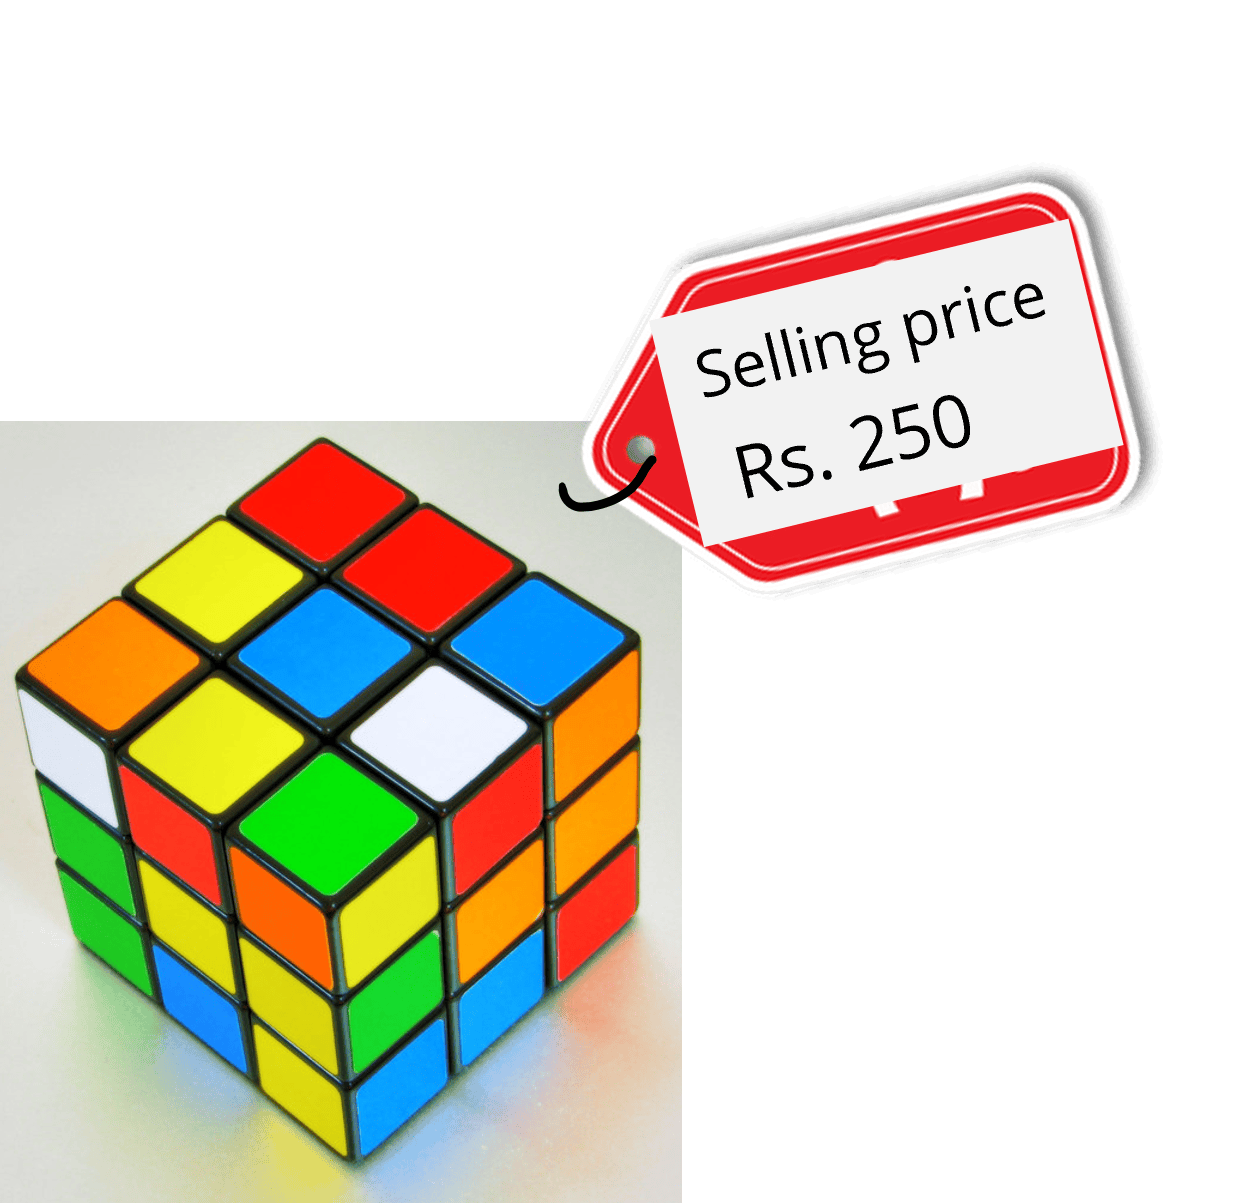
\includegraphics[width=4.5cm, height=3cm]{C7M09 - DT - Q10.png}} },
  optionA={Rs. 100},
  optionB={Rs. 350},
  optionC={Rs. 250},
  optionD={Rs. 150},
  correctoption={D},
  leftmini={0.5},
  rightmini={0.4},
}

\begin{minipage}{\linewidth}
\hspace{1cm}
\centering
\tiny
\renewcommand{\arraystretch}{1.25}
\begin{tabular}{|M{1.2cm}|M{0.8cm}|M{0.8cm}|M{0.8cm}|M{0.8cm}|M{0.8cm}|}
\hline
Option & A (\ding{55}) & B (\ding{55}) & C (\ding{55}) & \cellcolor{cellgreen} D (\ding{51}) & E \\ 
\hline
7 A & \highno{6\%} & \highno{6\%} & \highno{6\%} & \highno{75\%} & \highno{6\%} \\ 
 \hline 
7 B & \highno{7\%} & \highno{7\%} & \highno{7\%} & \highno{71\%} & \highno{7\%} \\ \hline
\end{tabular}
\end{minipage}

\end{frame}
% \input{4. PPT/My Answer/Math/C7/117_C7M - Q13}


\begin{frame}[shrink=0.1,label=QPC7QC7M09 - DT - Q8]{Q18 [7. Comparing Quantities]}
\vspace{-0.2cm}
\mcqtextbottomOneFour{
  questionnumber={18}, 
  questionTag={C7M09 – DT – Q8}, 
  questiontext={If Shalu ate 20 chocolates out of 80, what would be the percentage of the chocolates eaten by her?},
  optionA={25\%},
  optionB={4\%},
  optionC={20\%},
  optionD={60\%},
  correctoption={A},
}

\begin{minipage}{\linewidth}
\hspace{1cm}
\centering
\tiny
\renewcommand{\arraystretch}{1.25}
\begin{tabular}{|M{1.2cm}|M{0.8cm}|M{0.8cm}|M{0.8cm}|M{0.8cm}|M{0.8cm}|}
\hline
Option & \cellcolor{cellgreen} A (\ding{51}) & B (\ding{55}) & C (\ding{55}) & D (\ding{55}) & E \\ 
\hline
7 A & \highred{19\%} & \highno{25\%} & \highno{19\%} & \highno{31\%} & \highno{6\%} \\ 
 \hline 
7 B & \highred{21\%} & \highno{21\%} & \highno{36\%} & \highno{21\%} & \highno{0\%} \\ \hline
\end{tabular}
\end{minipage}

\end{frame}
% \input{4. PPT/My Answer/Math/C7/117_C7M - Q18}


\begin{frame}[shrink=0.1,label=QPC7QC7M09 - DT - Q3]{Q22 [7. Comparing Quantities]}
\vspace{-0.2cm}
\mcqtextbottomOneFour{
  questionnumber={22}, 
  questionTag={C7M09 – DT – Q3}, 
  questiontext={If 10 apples cost Rs. 100, what will be the price of 6 apples?},
  optionA={Rs. 50},
  optionB={Rs. 100},
  optionC={Rs. 600},
  optionD={Rs. 60},
  correctoption={D},
}

\begin{minipage}{\linewidth}
\hspace{1cm}
\centering
\tiny
\renewcommand{\arraystretch}{1.25}
\begin{tabular}{|M{1.2cm}|M{0.8cm}|M{0.8cm}|M{0.8cm}|M{0.8cm}|M{0.8cm}|}
\hline
Option & A (\ding{55}) & B (\ding{55}) & C (\ding{55}) & \cellcolor{cellgreen} D (\ding{51}) & E \\ 
\hline
7 A & \highno{6\%} & \highno{0\%} & \highno{13\%} & \highgreen{81\%} & \highno{0\%} \\ 
 \hline 
7 B & \highno{7\%} & \highno{0\%} & \highno{7\%} & \highgreen{86\%} & \highno{0\%} \\ \hline
\end{tabular}
\end{minipage}

\end{frame}
% \input{4. PPT/My Answer/Math/C7/117_C7M - Q22}


\begin{frame}[shrink=0.1,label=QPC7QC7M09 - DT - Q5]{Q25 [7. Comparing Quantities]}
\vspace{-0.2cm}
\mcqtextbottomOneFour{
  questionnumber={25}, 
  questionTag={C7M09 – DT – Q5}, 
  questiontext={Convert the following fraction into a percentage. \quad {{$\dfrac{5}{7}$}}},
  optionA={0.714\%},
  optionB={70.4\%},
  optionC={0.0074\%},
  optionD={71.4\%},
  correctoption={D},
}

\begin{minipage}{\linewidth}
\hspace{1cm}
\centering
\tiny
\renewcommand{\arraystretch}{1.25}
\begin{tabular}{|M{1.2cm}|M{0.8cm}|M{0.8cm}|M{0.8cm}|M{0.8cm}|M{0.8cm}|}
\hline
Option & A (\ding{55}) & B (\ding{55}) & C (\ding{55}) & \cellcolor{cellgreen} D (\ding{51}) & E \\ 
\hline
7 A & \highno{0\%} & \highno{38\%} & \highno{13\%} & \highred{25\%} & \highno{25\%} \\ 
 \hline 
7 B & \highno{7\%} & \highno{21\%} & \highno{14\%} & \highred{36\%} & \highno{21\%} \\ \hline
\end{tabular}
\end{minipage}

\end{frame}
% \input{4. PPT/My Answer/Math/C7/117_C7M - Q25}


\begin{frame}[shrink=0.1,label=QPC7QC7M09 - DT - Q14]{Q40 [7. Comparing Quantities]}
\vspace{-0.2cm}
\mcqtextbottomOneFour{
  questionnumber={40}, 
  questionTag={C7M09 - DT - Q14}, 
  questiontext={If the principle is Rs. 100 and the rate is 2\%, what will be the amount after 3 years?},
  optionA={Rs. 105},
  optionB={Rs. 106},
  optionC={Rs. 103},
  optionD={Rs. 6},
  correctoption={B},
}

\begin{minipage}{\linewidth}
\hspace{1cm}
\centering
\tiny
\renewcommand{\arraystretch}{1.25}
\begin{tabular}{|M{1.2cm}|M{0.8cm}|M{0.8cm}|M{0.8cm}|M{0.8cm}|M{0.8cm}|}
\hline
Option & A (\ding{55}) & \cellcolor{cellgreen} B (\ding{51}) & C (\ding{55}) & D (\ding{55}) & E \\ 
\hline
7 A & \highno{19\%} & \highred{25\%} & \highno{13\%} & \highno{44\%} & \highno{0\%} \\ 
 \hline 
7 B & \highno{14\%} & \highred{21\%} & \highno{14\%} & \highno{50\%} & \highno{0\%} \\ \hline
\end{tabular}
\end{minipage}

\end{frame}
% \input{4. PPT/My Answer/Math/C7/117_C7M - Q40}


\begin{frame}[shrink=0.1,label=QPC7QC7M09 - CT - Q1]{Q60 [7. Comparing Quantities]}
\vspace{-0.2cm}
\mcqtextbottomOneFour{
  questionnumber={60 - Critical Thinking},
  questionTag = {C7M09 - CT - Q1},
  questiontext = {Ben distributed different varieties of vegetables to his friends.\\
  \begin{table}[H]
      \centering
      \renewcommand{\arraystretch}{1.5}
      \begin{tabular}{|c|c|c|c|}
          \hline
          Carrot  & Beetroot &Potato & Cucumber  \\
          \hline
          60\% of 2 kg& 39\% of 2 kg & 76\% of 2 kg &25\% of 2 kg\\
          \hline
      \end{tabular}
  \end{table}
  Find the total kilogram of vegetables shared with his friends.},
  optionA={2},
  optionB={4},
  optionC={8},
  optionD={5.5},
  correctoption = {B},
  }

\begin{minipage}{\linewidth}
\hspace{1cm}
\centering
\tiny
\renewcommand{\arraystretch}{1.25}
\begin{tabular}{|M{1.2cm}|M{0.8cm}|M{0.8cm}|M{0.8cm}|M{0.8cm}|M{0.8cm}|}
\hline
Option & A (\ding{55}) & \cellcolor{cellgreen} B (\ding{51}) & C (\ding{55}) & D (\ding{55}) & E \\ 
\hline
7 A & \highno{19\%} & \highred{13\%} & \highno{56\%} & \highno{13\%} & \highno{0\%} \\ 
 \hline 
7 B & \highno{14\%} & \highred{21\%} & \highno{43\%} & \highno{21\%} & \highno{0\%} \\ \hline
\end{tabular}
\end{minipage}

\end{frame}
% \input{4. PPT/My Answer/Math/C7/117_C7M - Q60 - Critical Thinking}


\begin{frame}[shrink=0.1,label=QPC7QC7M04 - DT - Q2]{Q6 [8. Rational Numbers]}
\vspace{-0.2cm}
\mcqtextbottomOneFour{
  questionnumber={6}, 
  questionTag={C7M04 – DT – Q2}, 
  questiontext={If {{$\dfrac{p}{q}$}} is a rational number, then \rule{40pt}{0.5pt}.},
  optionA={p $=$ not defined},
  optionB={q $\neq$ 0},
  optionC={q $=$ 0},
  optionD={None of the above},
  correctoption={B},
}

\begin{minipage}{\linewidth}
\hspace{1cm}
\centering
\tiny
\renewcommand{\arraystretch}{1.25}
\begin{tabular}{|M{1.2cm}|M{0.8cm}|M{0.8cm}|M{0.8cm}|M{0.8cm}|M{0.8cm}|}
\hline
Option & A (\ding{55}) & \cellcolor{cellgreen} B (\ding{51}) & C (\ding{55}) & D (\ding{55}) & E \\ 
\hline
7 A & \highno{0\%} & \highno{75\%} & \highno{25\%} & \highno{0\%} & \highno{0\%} \\ 
 \hline 
7 B & \highno{7\%} & \highgreen{86\%} & \highno{0\%} & \highno{7\%} & \highno{0\%} \\ \hline
\end{tabular}
\end{minipage}

\end{frame}
% \input{4. PPT/My Answer/Math/C7/117_C7M - Q6}


\begin{frame}[shrink=0.1,label=QPC7QC7M04 - DT - Q6]{Q21 [8. Rational Numbers]}
\vspace{-0.2cm}
\mcqtextbottomOneFour{
 questionnumber={21}, 
  questionTag={C7M04 – DT – Q6}, 
  questiontext={Find the standard form of {{$\dfrac{20}{80}$}}.},
  optionA={{{$\dfrac{10}{40}$}} },
  optionB={{{$\dfrac{2}{8}$}} },
  optionC={ {{$\dfrac{200}{800}$}} },
  optionD={ {{$\dfrac{1}{4}$}} },
  correctoption={D},
}

\begin{minipage}{\linewidth}
\hspace{1cm}
\centering
\tiny
\renewcommand{\arraystretch}{1.25}
\begin{tabular}{|M{1.2cm}|M{0.8cm}|M{0.8cm}|M{0.8cm}|M{0.8cm}|M{0.8cm}|}
\hline
Option & A (\ding{55}) & B (\ding{55}) & C (\ding{55}) & \cellcolor{cellgreen} D (\ding{51}) & E \\ 
\hline
7 A & \highno{6\%} & \highno{31\%} & \highno{13\%} & \highno{50\%} & \highno{0\%} \\ 
 \hline 
7 B & \highno{14\%} & \highno{36\%} & \highno{0\%} & \highno{50\%} & \highno{0\%} \\ \hline
\end{tabular}
\end{minipage}

\end{frame}
% \input{4. PPT/My Answer/Math/C7/117_C7M - Q21}


\begin{frame}[shrink=0.1,label=QPC7QC7M04 - DT - Q7]{Q50 [8. Rational Numbers]}
\vspace{-0.2cm}
\mcqtextbottomOneFour{
 questionnumber={50}, 
  questionTag={C7M04 – DT – Q7}, 
  questiontext={Compare: {{$\dfrac{7}{5}$}} \boxed{\color{white}AA} {{$\dfrac{18}{15}$}}.},
  optionA={$=$ },
  optionB={$>$ },
  optionC={$<$ },
  optionD={None of these},
  correctoption={B},
}

\begin{minipage}{\linewidth}
\hspace{1cm}
\centering
\tiny
\renewcommand{\arraystretch}{1.25}
\begin{tabular}{|M{1.2cm}|M{0.8cm}|M{0.8cm}|M{0.8cm}|M{0.8cm}|M{0.8cm}|}
\hline
Option & A (\ding{55}) & \cellcolor{cellgreen} B (\ding{51}) & C (\ding{55}) & D (\ding{55}) & E \\ 
\hline
7 A & \highno{0\%} & \highno{75\%} & \highno{19\%} & \highno{0\%} & \highno{6\%} \\ 
 \hline 
7 B & \highno{0\%} & \highno{57\%} & \highno{43\%} & \highno{0\%} & \highno{0\%} \\ \hline
\end{tabular}
\end{minipage}

\end{frame}
% \input{4. PPT/My Answer/Math/C7/117_C7M - Q50}


\begin{frame}[shrink=0.1,label=QPC7QC7M04 - DT - Q9]{Q51 [8. Rational Numbers]}
\vspace{-0.2cm}
\mcqtextbottomOneFour{
 questionnumber={51}, 
  questionTag={C7M04 – DT – Q9}, 
  questiontext={Solve:$ -${{$\dfrac{6}{7}$}} $\times$ 12.},
  optionA={$ -$ {{$\dfrac{6}{84}$}} },
  optionB={$ -$ {{$\dfrac{72}{84}$}} },
  optionC={$ -$ {{$\dfrac{2}{7}$}} },
  optionD={$ -$ {{$\dfrac{72}{7}$}} },
  correctoption={D},
}

\begin{minipage}{\linewidth}
\hspace{1cm}
\centering
\tiny
\renewcommand{\arraystretch}{1.25}
\begin{tabular}{|M{1.2cm}|M{0.8cm}|M{0.8cm}|M{0.8cm}|M{0.8cm}|M{0.8cm}|}
\hline
Option & A (\ding{55}) & B (\ding{55}) & C (\ding{55}) & \cellcolor{cellgreen} D (\ding{51}) & E \\ 
\hline
7 A & \highno{13\%} & \highno{25\%} & \highno{13\%} & \highno{44\%} & \highno{6\%} \\ 
 \hline 
7 B & \highno{7\%} & \highno{21\%} & \highno{7\%} & \highno{64\%} & \highno{0\%} \\ \hline
\end{tabular}
\end{minipage}

\end{frame}
% \input{4. PPT/My Answer/Math/C7/117_C7M - Q51}


\begin{frame}[shrink=0.1,label=QPC7QC7M16 - DT - Q1]{Q27 [9. Perimeter and Area]}
\vspace{-0.2cm}
\mcqtextbottomOneFour{
  questionnumber={27}, 
  questionTag={C7M16 – DT – Q1}, 
  questiontext={$(4 \times$ length of a side) is the perimeter of a \rule{80pt}{0.1pt}.},
  optionA={Parallelogram},
  optionB={Square},
  optionC={ Rectangle},
  optionD={ Triangle},
  correctoption={B},
}

\begin{minipage}{\linewidth}
\hspace{1cm}
\centering
\tiny
\renewcommand{\arraystretch}{1.25}
\begin{tabular}{|M{1.2cm}|M{0.8cm}|M{0.8cm}|M{0.8cm}|M{0.8cm}|M{0.8cm}|}
\hline
Option & A (\ding{55}) & \cellcolor{cellgreen} B (\ding{51}) & C (\ding{55}) & D (\ding{55}) & E \\ 
\hline
7 A & \highno{0\%} & \highgreen{88\%} & \highno{13\%} & \highno{0\%} & \highno{0\%} \\ 
 \hline 
7 B & \highno{0\%} & \highgreen{93\%} & \highno{0\%} & \highno{0\%} & \highno{7\%} \\ \hline
\end{tabular}
\end{minipage}

\end{frame}
% \input{4. PPT/My Answer/Math/C7/117_C7M - Q27}


\begin{frame}[shrink=0.1,label=QPC7QC7M16 - DT - Q7]{Q28 [9. Perimeter and Area]}
\vspace{-0.2cm}
\mcqtextbottomOneFour{
  questionnumber={28}, 
  questionTag={C7M16 – DT – Q7}, 
  questiontext={Find the area of the circle, if the diameter is 14 cm.},
  optionA={88 cm$^2$},
  optionB={616 cm$^2$},
  optionC={154 cm$^2$},
  optionD={196 cm$^2$},
  correctoption={C},
}

\begin{minipage}{\linewidth}
\hspace{1cm}
\centering
\tiny
\renewcommand{\arraystretch}{1.25}
\begin{tabular}{|M{1.2cm}|M{0.8cm}|M{0.8cm}|M{0.8cm}|M{0.8cm}|M{0.8cm}|}
\hline
Option & A (\ding{55}) & B (\ding{55}) & \cellcolor{cellgreen} C (\ding{51}) & D (\ding{55}) & E \\ 
\hline
7 A & \highno{6\%} & \highno{38\%} & \highred{38\%} & \highno{13\%} & \highno{6\%} \\ 
 \hline 
7 B & \highno{7\%} & \highno{43\%} & \highred{36\%} & \highno{14\%} & \highno{0\%} \\ \hline
\end{tabular}
\end{minipage}

\end{frame}
% \input{4. PPT/My Answer/Math/C7/117_C7M - Q28}


\begin{frame}[shrink=0.1,label=QPC7QC7M16 - DT - Q3]{Q35 [9. Perimeter and Area]}
\vspace{-0.2cm}
\mcqtextbottomOneFour{
  questionnumber={35}, 
  questionTag={C7M16 – DT – Q3}, 
  questiontext={If a parallelogram has a base of 11 cm and a height of 4 cm, find whose statement is correct.\\ Vinith: Area of the parallelogram is 44 cm$^2$.\\ Nirvitha: Area of the parallelogram is 44 cm.},
  optionA={Vinith},
  optionB={Nirvitha},
  optionC={ Both of them},
  optionD={ None of them},
  correctoption={A},
}

\begin{minipage}{\linewidth}
\hspace{1cm}
\centering
\tiny
\renewcommand{\arraystretch}{1.25}
\begin{tabular}{|M{1.2cm}|M{0.8cm}|M{0.8cm}|M{0.8cm}|M{0.8cm}|M{0.8cm}|}
\hline
Option & \cellcolor{cellgreen} A (\ding{51}) & B (\ding{55}) & C (\ding{55}) & D (\ding{55}) & E \\ 
\hline
7 A & \highno{75\%} & \highno{6\%} & \highno{6\%} & \highno{13\%} & \highno{0\%} \\ 
 \hline 
7 B & \highno{50\%} & \highno{21\%} & \highno{14\%} & \highno{7\%} & \highno{7\%} \\ \hline
\end{tabular}
\end{minipage}

\end{frame}
% \input{4. PPT/My Answer/Math/C7/117_C7M - Q35}


\begin{frame}[shrink=0.1,label=QPC7QC7M16 - DT - Q2]{Q43 [9. Perimeter and Area]}
\vspace{-0.2cm}
\mcqimgleftFourOne{
  questionnumber={43}, 
  questionTag={C7M16 – DT – Q2},
  questiontext={Find the area of the given rectangular card.},
  imgtabletikz = { 
\tikzset{every picture/.style={line width=0.75pt,scale=\scalefactor}} 
\hspace{3cm}
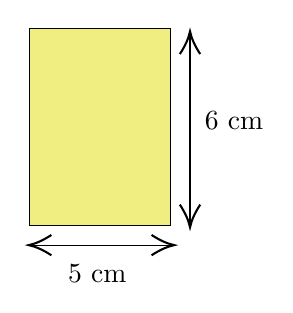
\begin{tikzpicture}[x=0.75pt,y=0.75pt,yscale=-1,xscale=1]
\draw  [fill={rgb, 255:red, 240; green, 237; blue, 129 }  ,fill opacity=1 ] (220.01,27.02) -- (288.23,27.02) -- (288.23,122.08) -- (220.01,122.08) -- cycle ;
\draw    (297.52,30.53) -- (297.52,120.94) ;
\draw [shift={(297.52,122.94)}, rotate = 270] [color={rgb, 255:red, 0; green, 0; blue, 0 }  ][line width=0.75]    (10.93,-4.9) .. controls (6.95,-2.3) and (3.31,-0.67) .. (0,0) .. controls (3.31,0.67) and (6.95,2.3) .. (10.93,4.9)   ;
\draw [shift={(297.52,28.53)}, rotate = 90] [color={rgb, 255:red, 0; green, 0; blue, 0 }  ][line width=0.75]    (10.93,-4.9) .. controls (6.95,-2.3) and (3.31,-0.67) .. (0,0) .. controls (3.31,0.67) and (6.95,2.3) .. (10.93,4.9)   ;
\draw    (221.8,131.52) -- (253.59,131.52) -- (287.92,131.52) ;
\draw [shift={(289.92,131.52)}, rotate = 180] [color={rgb, 255:red, 0; green, 0; blue, 0 }  ][line width=0.75]    (10.93,-4.9) .. controls (6.95,-2.3) and (3.31,-0.67) .. (0,0) .. controls (3.31,0.67) and (6.95,2.3) .. (10.93,4.9)   ;
\draw [shift={(219.8,131.52)}, rotate = 0] [color={rgb, 255:red, 0; green, 0; blue, 0 }  ][line width=0.75]    (10.93,-4.9) .. controls (6.95,-2.3) and (3.31,-0.67) .. (0,0) .. controls (3.31,0.67) and (6.95,2.3) .. (10.93,4.9)   ;
\draw (303.36,65.83) node [anchor=north west][inner sep=0.75pt]   [align=left] {6 cm};
\draw (237.47,139.64) node [anchor=north west][inner sep=0.75pt]   [align=left] {5 cm};
\end{tikzpicture}
  },
  optionA={65 cm},
  optionB={11 cm},
  optionC={22 cm$^2$},
  optionD={30 cm$^2$},
  correctoption={D},
  leftmini={0.5},
  rightmini={0.4},
}

\begin{minipage}{\linewidth}
\hspace{1cm}
\centering
\tiny
\renewcommand{\arraystretch}{1.25}
\begin{tabular}{|M{1.2cm}|M{0.8cm}|M{0.8cm}|M{0.8cm}|M{0.8cm}|M{0.8cm}|}
\hline
Option & A (\ding{55}) & B (\ding{55}) & C (\ding{55}) & \cellcolor{cellgreen} D (\ding{51}) & E \\ 
\hline
7 A & \highno{6\%} & \highno{13\%} & \highno{0\%} & \highgreen{81\%} & \highno{0\%} \\ 
 \hline 
7 B & \highno{7\%} & \highno{14\%} & \highno{36\%} & \highno{43\%} & \highno{0\%} \\ \hline
\end{tabular}
\end{minipage}

\end{frame}
% \input{4. PPT/My Answer/Math/C7/117_C7M - Q43}


\begin{frame}[shrink=0.1,label=QPC7QC7M08 - DT - Q6]{Q8 [10. Algebraic Expressions]}
\vspace{-0.2cm}
\mcqtextbottomOneFour{
  questionnumber={8}, 
  questionTag={C7M08 – DT – Q6}, 
  questiontext={$a^2 + 2ab + b^2$ is a \rule{40pt}{0.5pt} expression.},
  optionA={Monomial},
  optionB={Binomial},
  optionC={Trinomial},
  optionD={Not an expression},
  correctoption={C},
}

\begin{minipage}{\linewidth}
\hspace{1cm}
\centering
\tiny
\renewcommand{\arraystretch}{1.25}
\begin{tabular}{|M{1.2cm}|M{0.8cm}|M{0.8cm}|M{0.8cm}|M{0.8cm}|M{0.8cm}|}
\hline
Option & A (\ding{55}) & B (\ding{55}) & \cellcolor{cellgreen} C (\ding{51}) & D (\ding{55}) & E \\ 
\hline
7 A & \highno{6\%} & \highno{6\%} & \highred{19\%} & \highno{0\%} & \highno{69\%} \\ 
 \hline 
7 B & \highno{0\%} & \highno{7\%} & \highred{14\%} & \highno{0\%} & \highno{79\%} \\ \hline
\end{tabular}
\end{minipage}

\end{frame}
% \input{4. PPT/My Answer/Math/C7/117_C7M - Q8}


\begin{frame}[shrink=0.1,label=QPC7QC7M08 - DT - Q8]{Q15 [10. Algebraic Expressions]}
\vspace{-0.2cm}
\mcqtextbottomOneFour{
  questionnumber={15}, 
  questionTag={C7M08 – DT – Q8}, 
  questiontext={If r = 9, the value of the expression $r^2 + r - 9$ is \rule{40pt}{0.5pt} .},
  optionA={9},
  optionB={81},
  optionC={$-$9},
  optionD={0},
  correctoption={B},
}

\begin{minipage}{\linewidth}
\hspace{1cm}
\centering
\tiny
\renewcommand{\arraystretch}{1.25}
\begin{tabular}{|M{1.2cm}|M{0.8cm}|M{0.8cm}|M{0.8cm}|M{0.8cm}|M{0.8cm}|}
\hline
Option & A (\ding{55}) & \cellcolor{cellgreen} B (\ding{51}) & C (\ding{55}) & D (\ding{55}) & E \\ 
\hline
7 A & \highno{0\%} & \highno{63\%} & \highno{6\%} & \highno{19\%} & \highno{13\%} \\ 
 \hline 
7 B & \highno{0\%} & \highgreen{79\%} & \highno{7\%} & \highno{14\%} & \highno{0\%} \\ \hline
\end{tabular}
\end{minipage}

\end{frame}
% \input{4. PPT/My Answer/Math/C7/117_C7M - Q15}


\begin{frame}[shrink=0.1,label=QPC7QC7M08 - DT - Q2]{Q36 [10. Algebraic Expressions]}
\vspace{-0.2cm}
\mcqtextbottomOneFour{
  questionnumber={36}, 
  questionTag={C7M08 – DT – Q2}, 
  questiontext={Find the coefficient of $y$. \quad $y^2 +  6y + 3 = 0$},
  optionA={1},
  optionB={3},
  optionC={6},
  optionD={0},
  correctoption={C},
}

\begin{minipage}{\linewidth}
\hspace{1cm}
\centering
\tiny
\renewcommand{\arraystretch}{1.25}
\begin{tabular}{|M{1.2cm}|M{0.8cm}|M{0.8cm}|M{0.8cm}|M{0.8cm}|M{0.8cm}|}
\hline
Option & A (\ding{55}) & B (\ding{55}) & \cellcolor{cellgreen} C (\ding{51}) & D (\ding{55}) & E \\ 
\hline
7 A & \highno{6\%} & \highno{6\%} & \highgreen{88\%} & \highno{0\%} & \highno{0\%} \\ 
 \hline 
7 B & \highno{7\%} & \highno{7\%} & \highno{71\%} & \highno{7\%} & \highno{7\%} \\ \hline
\end{tabular}
\end{minipage}

\end{frame}
% \input{4. PPT/My Answer/Math/C7/117_C7M - Q36}


\begin{frame}[shrink=0.1,label=QPC7QC7M08 - DT - Q5]{Q57 [10. Algebraic Expressions]}
\vspace{-0.2cm}
\mcqtextbottomOneFour{
  questionnumber={57}, 
  questionTag={C7M08 – DT – Q5}, 
  questiontext={Solve: $(3a - 2b + c) - (2a - b + 2c)$},
  optionA={$a + b + c$},
  optionB={$a + 3b + 3c$},
  optionC={$a - b - c$},
  optionD={$a - b + c$},
  correctoption={C},
}

\begin{minipage}{\linewidth}
\hspace{1cm}
\centering
\tiny
\renewcommand{\arraystretch}{1.25}
\begin{tabular}{|M{1.2cm}|M{0.8cm}|M{0.8cm}|M{0.8cm}|M{0.8cm}|M{0.8cm}|}
\hline
Option & A (\ding{55}) & B (\ding{55}) & \cellcolor{cellgreen} C (\ding{51}) & D (\ding{55}) & E \\ 
\hline
7 A & \highno{0\%} & \highno{25\%} & \highred{13\%} & \highno{38\%} & \highno{25\%} \\ 
 \hline 
7 B & \highno{0\%} & \highno{43\%} & \highred{0\%} & \highno{57\%} & \highno{0\%} \\ \hline
\end{tabular}
\end{minipage}

\end{frame}
% \input{4. PPT/My Answer/Math/C7/117_C7M - Q57}


\begin{frame}[shrink=0.1,label=QPC7QC7M05 - DT - Q2]{Q29 [11. Exponents and Powers]}
\vspace{-0.2cm}
\mcqimgleftFourOne{
  questionnumber={29}, 
  questionTag={C7M05 – DT – Q2},
  questiontext={Match the following.},
  imgtabletikz = {

\begin{table}[H]
\centering
\renewcommand{\arraystretch}{1.15}
    \begin{tabular}{|p{0.5cm}|p{2cm}|p{0.2cm}|p{0.5cm}|p{2cm}|}
      \cline{1-5} 
       \multicolumn{2}{|c|}{\textbf{Column A }} & 
      \multirow{5}{*}{} &   
      \multicolumn{2}{c|}{\textbf{Column B}} \\
      \cline{1-2}\cline{4-5} i.  & $x^2 \times x^5$ &   & a. & $x^{2\times5}$ \\
      \cline{1-2}\cline{4-5} ii. & $x^2 \divisionsymbol x^5$ &   & b. &  $x^{2+5}$\\
      \cline{1-2}\cline{4-5} iii.  & $x^0 \times x^2$
 &   & c. & $x^{2-5}$ \\
  \cline{1-2}\cline{4-5} iv.  & $(x^2)^5$
 &   & d. & $x^2$ \\
 \hline
    \end{tabular}
\end{table}},
 optionA={i - b, ii - c, iii - a, iv - d},
  optionB={i - c, ii - b, iii - a, iv - d},
  optionC={i - b, ii - c, iii - d, iv - a},
  optionD={i - a, ii - c, iii - d, iv - b},
  correctoption={C},
  leftmini={0.5},
  rightmini={0.4},
}

\begin{minipage}{\linewidth}
\hspace{1cm}
\centering
\tiny
\renewcommand{\arraystretch}{1.25}
\begin{tabular}{|M{1.2cm}|M{0.8cm}|M{0.8cm}|M{0.8cm}|M{0.8cm}|M{0.8cm}|}
\hline
Option & A (\ding{55}) & B (\ding{55}) & \cellcolor{cellgreen} C (\ding{51}) & D (\ding{55}) & E \\ 
\hline
7 A & \highno{0\%} & \highno{13\%} & \highgreen{81\%} & \highno{6\%} & \highno{0\%} \\ 
 \hline 
7 B & \highno{7\%} & \highno{0\%} & \highgreen{86\%} & \highno{0\%} & \highno{7\%} \\ \hline
\end{tabular}
\end{minipage}

\end{frame}
% \input{4. PPT/My Answer/Math/C7/117_C7M - Q29}


\begin{frame}[shrink=0.1,label=QPC7QC7M05 - DT - Q1]{Q49 [11. Exponents and Powers]}
\vspace{-0.2cm}
\mcqtextbottomOneFour{
 questionnumber={49}, 
  questionTag={C7M05 – DT – Q1}, 
  questiontext={The result of $(-3)^2$ is \rule{40pt}{0.5pt}.},
  optionA={Positive number},
  optionB={Negative number},
  optionC={Zero },
  optionD={One },
  correctoption={A},
}

\begin{minipage}{\linewidth}
\hspace{1cm}
\centering
\tiny
\renewcommand{\arraystretch}{1.25}
\begin{tabular}{|M{1.2cm}|M{0.8cm}|M{0.8cm}|M{0.8cm}|M{0.8cm}|M{0.8cm}|}
\hline
Option & \cellcolor{cellgreen} A (\ding{51}) & B (\ding{55}) & C (\ding{55}) & D (\ding{55}) & E \\ 
\hline
7 A & \highno{50\%} & \highno{44\%} & \highno{0\%} & \highno{6\%} & \highno{0\%} \\ 
 \hline 
7 B & \highred{36\%} & \highno{50\%} & \highno{7\%} & \highno{0\%} & \highno{7\%} \\ \hline
\end{tabular}
\end{minipage}

\end{frame}
% \input{4. PPT/My Answer/Math/C7/117_C7M - Q49}


\begin{frame}[shrink=0.1,label=QPC7QC7M13 - DT - Q3]{Q7 [12. Symmetry]}
\vspace{-0.2cm}
\mcqtextbottomOneFour{
  questionnumber={7}, 
  questionTag={C7M13 - DT - Q3}, 
  questiontext={Find the mirror image of the given image. (Hint: Tortoise is standing on the mirror).\\
  \centering {\adjustbox{scale=\scalefactor}{
\includegraphics[width=75pt,height=45pt]{C7M13 - DT - Q3i.png }}}
  },
  optionA={{\adjustbox{scale=\scalefactor}{
\includegraphics[width=75pt,height=45pt]{C7M13 - DT - Q3i.png }}}},
  optionB={{\adjustbox{scale=\scalefactor}{
\includegraphics[width=75pt,height=45pt]{C7M13 - DT - Q3ii.png}} }},
  optionC={{\adjustbox{scale=\scalefactor}{
\includegraphics[width=75pt,height=45pt]{C7M13 - DT - Q3iv.png}} }},
  optionD={{\adjustbox{scale=\scalefactor}{
\includegraphics[width=55pt,height=65pt]{C7M13 - DT - Q3iii.png}} }},
  correctoption={B},
}

\begin{minipage}{\linewidth}
\hspace{1cm}
\centering
\tiny
\renewcommand{\arraystretch}{1.25}
\begin{tabular}{|M{1.2cm}|M{0.8cm}|M{0.8cm}|M{0.8cm}|M{0.8cm}|M{0.8cm}|}
\hline
Option & A (\ding{55}) & \cellcolor{cellgreen} B (\ding{51}) & C (\ding{55}) & D (\ding{55}) & E \\ 
\hline
7 A & \highno{13\%} & \highred{25\%} & \highno{63\%} & \highno{0\%} & \highno{0\%} \\ 
 \hline 
7 B & \highno{7\%} & \highred{29\%} & \highno{64\%} & \highno{0\%} & \highno{0\%} \\ \hline
\end{tabular}
\end{minipage}

\end{frame}
% \input{4. PPT/My Answer/Math/C7/117_C7M - Q7}


\begin{frame}[shrink=0.1,label=QPC7QC7M13 - DT - Q4]{Q19 [12. Symmetry]}
\vspace{-0.2cm}
\mcqtextbottomOneFour{
  questionnumber={19}, 
  questionTag={C7M13 - DT - Q4}, 
  questiontext={Identify the shape that has rotational symmetry of order 2.},
  optionA={
\tikzset{every picture/.style={line width=0.75pt,scale=\scalefactor}}
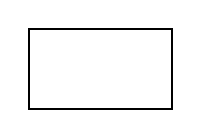
\begin{tikzpicture}[x=0.75pt,y=0.75pt,yscale=-1,xscale=1]
\draw  [line width=0.75]  (121,140.53) -- (190,140.53) -- (190,179.27) -- (121,179.27) -- cycle ;
\end{tikzpicture} },
  optionB={\tikzset{every picture/.style={line width=0.75pt,scale=\scalefactor}} 
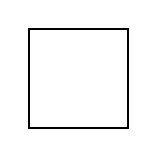
\begin{tikzpicture}[x=0.75pt,y=0.75pt,yscale=-1,xscale=1]\draw  [line width=0.75]  (118.28,125.72) -- (166.28,125.72) -- (166.28,173.72) -- (118.28,173.72) -- cycle ;
\end{tikzpicture}},
  optionC={
\tikzset{every picture/.style={line width=0.75pt,scale=\scalefactor}} 
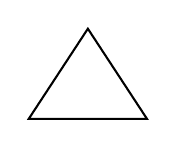
\begin{tikzpicture}[x=0.75pt,y=0.75pt,yscale=-1,xscale=1]
\draw  [line width=0.75]  (128.5,158.55) -- (157,202) -- (100,202) -- cycle ;
\end{tikzpicture} },
  optionD={Both a and c},
  correctoption={A},
}

\begin{minipage}{\linewidth}
\hspace{1cm}
\centering
\tiny
\renewcommand{\arraystretch}{1.25}
\begin{tabular}{|M{1.2cm}|M{0.8cm}|M{0.8cm}|M{0.8cm}|M{0.8cm}|M{0.8cm}|}
\hline
Option & \cellcolor{cellgreen} A (\ding{51}) & B (\ding{55}) & C (\ding{55}) & D (\ding{55}) & E \\ 
\hline
7 A & \highred{6\%} & \highno{38\%} & \highno{19\%} & \highno{31\%} & \highno{6\%} \\ 
 \hline 
7 B & \highred{14\%} & \highno{14\%} & \highno{0\%} & \highno{71\%} & \highno{0\%} \\ \hline
\end{tabular}
\end{minipage}

\end{frame}
% \input{4. PPT/My Answer/Math/C7/117_C7M - Q19}


\begin{frame}[shrink=0.1,label=QPC7QC7M13 - DT - Q7]{Q34 [12. Symmetry]}
\vspace{-0.2cm}
\mcqtextbottomOneFour{
  questionnumber={34}, 
  questionTag={C7M13 - DT - Q7}, 
  questiontext={ Find which of the alphabet has two lines of symmetry. },
  optionA={B},
  optionB={C},
  optionC={N},
  optionD={X},
  correctoption={D},
}

\begin{minipage}{\linewidth}
\hspace{1cm}
\centering
\tiny
\renewcommand{\arraystretch}{1.25}
\begin{tabular}{|M{1.2cm}|M{0.8cm}|M{0.8cm}|M{0.8cm}|M{0.8cm}|M{0.8cm}|}
\hline
Option & A (\ding{55}) & B (\ding{55}) & C (\ding{55}) & \cellcolor{cellgreen} D (\ding{51}) & E \\ 
\hline
7 A & \highno{13\%} & \highno{6\%} & \highno{6\%} & \highno{75\%} & \highno{0\%} \\ 
 \hline 
7 B & \highno{7\%} & \highno{7\%} & \highno{14\%} & \highno{64\%} & \highno{7\%} \\ \hline
\end{tabular}
\end{minipage}

\end{frame}
% \input{4. PPT/My Answer/Math/C7/117_C7M - Q34}


\begin{frame}[shrink=0.1,label=QPC7QC7M14 - DT - Q1]{Q10 [13. Visualising Solid Shapes]}
\vspace{-0.2cm}
\mcqtextbottomOneFour{
  questionnumber={10}, 
  questionTag={C7M14 - DT - Q1}, 
  questiontext={The 3D representation of a square is a \rule{30pt}{0.5pt}.  },
  optionA={Cuboid},
  optionB={Cylinder},
  optionC={Cone},
  optionD={Cube},
  correctoption={D},
}

\begin{minipage}{\linewidth}
\hspace{1cm}
\centering
\tiny
\renewcommand{\arraystretch}{1.25}
\begin{tabular}{|M{1.2cm}|M{0.8cm}|M{0.8cm}|M{0.8cm}|M{0.8cm}|M{0.8cm}|}
\hline
Option & A (\ding{55}) & B (\ding{55}) & C (\ding{55}) & \cellcolor{cellgreen} D (\ding{51}) & E \\ 
\hline
7 A & \highno{19\%} & \highno{0\%} & \highno{6\%} & \highno{75\%} & \highno{0\%} \\ 
 \hline 
7 B & \highno{14\%} & \highno{0\%} & \highno{21\%} & \highno{64\%} & \highno{0\%} \\ \hline
\end{tabular}
\end{minipage}

\end{frame}
% \input{4. PPT/My Answer/Math/C7/117_C7M - Q10}


\begin{frame}[shrink=0.1,label=QPC7QC7M14 - DT - Q5]{Q17 [13. Visualising Solid Shapes]}
\vspace{-0.2cm}
\mcqimgleftFourOne{
  questionnumber={17}, 
  questionTag={C7M14 - DT - Q5}, 
  questiontext={Kevin arranged the cubes in the table as shown below. How many cubes are visible when the cubes are viewed from the top view?},
  imgtabletikz = { \adjustbox{scale=\scalefactor}{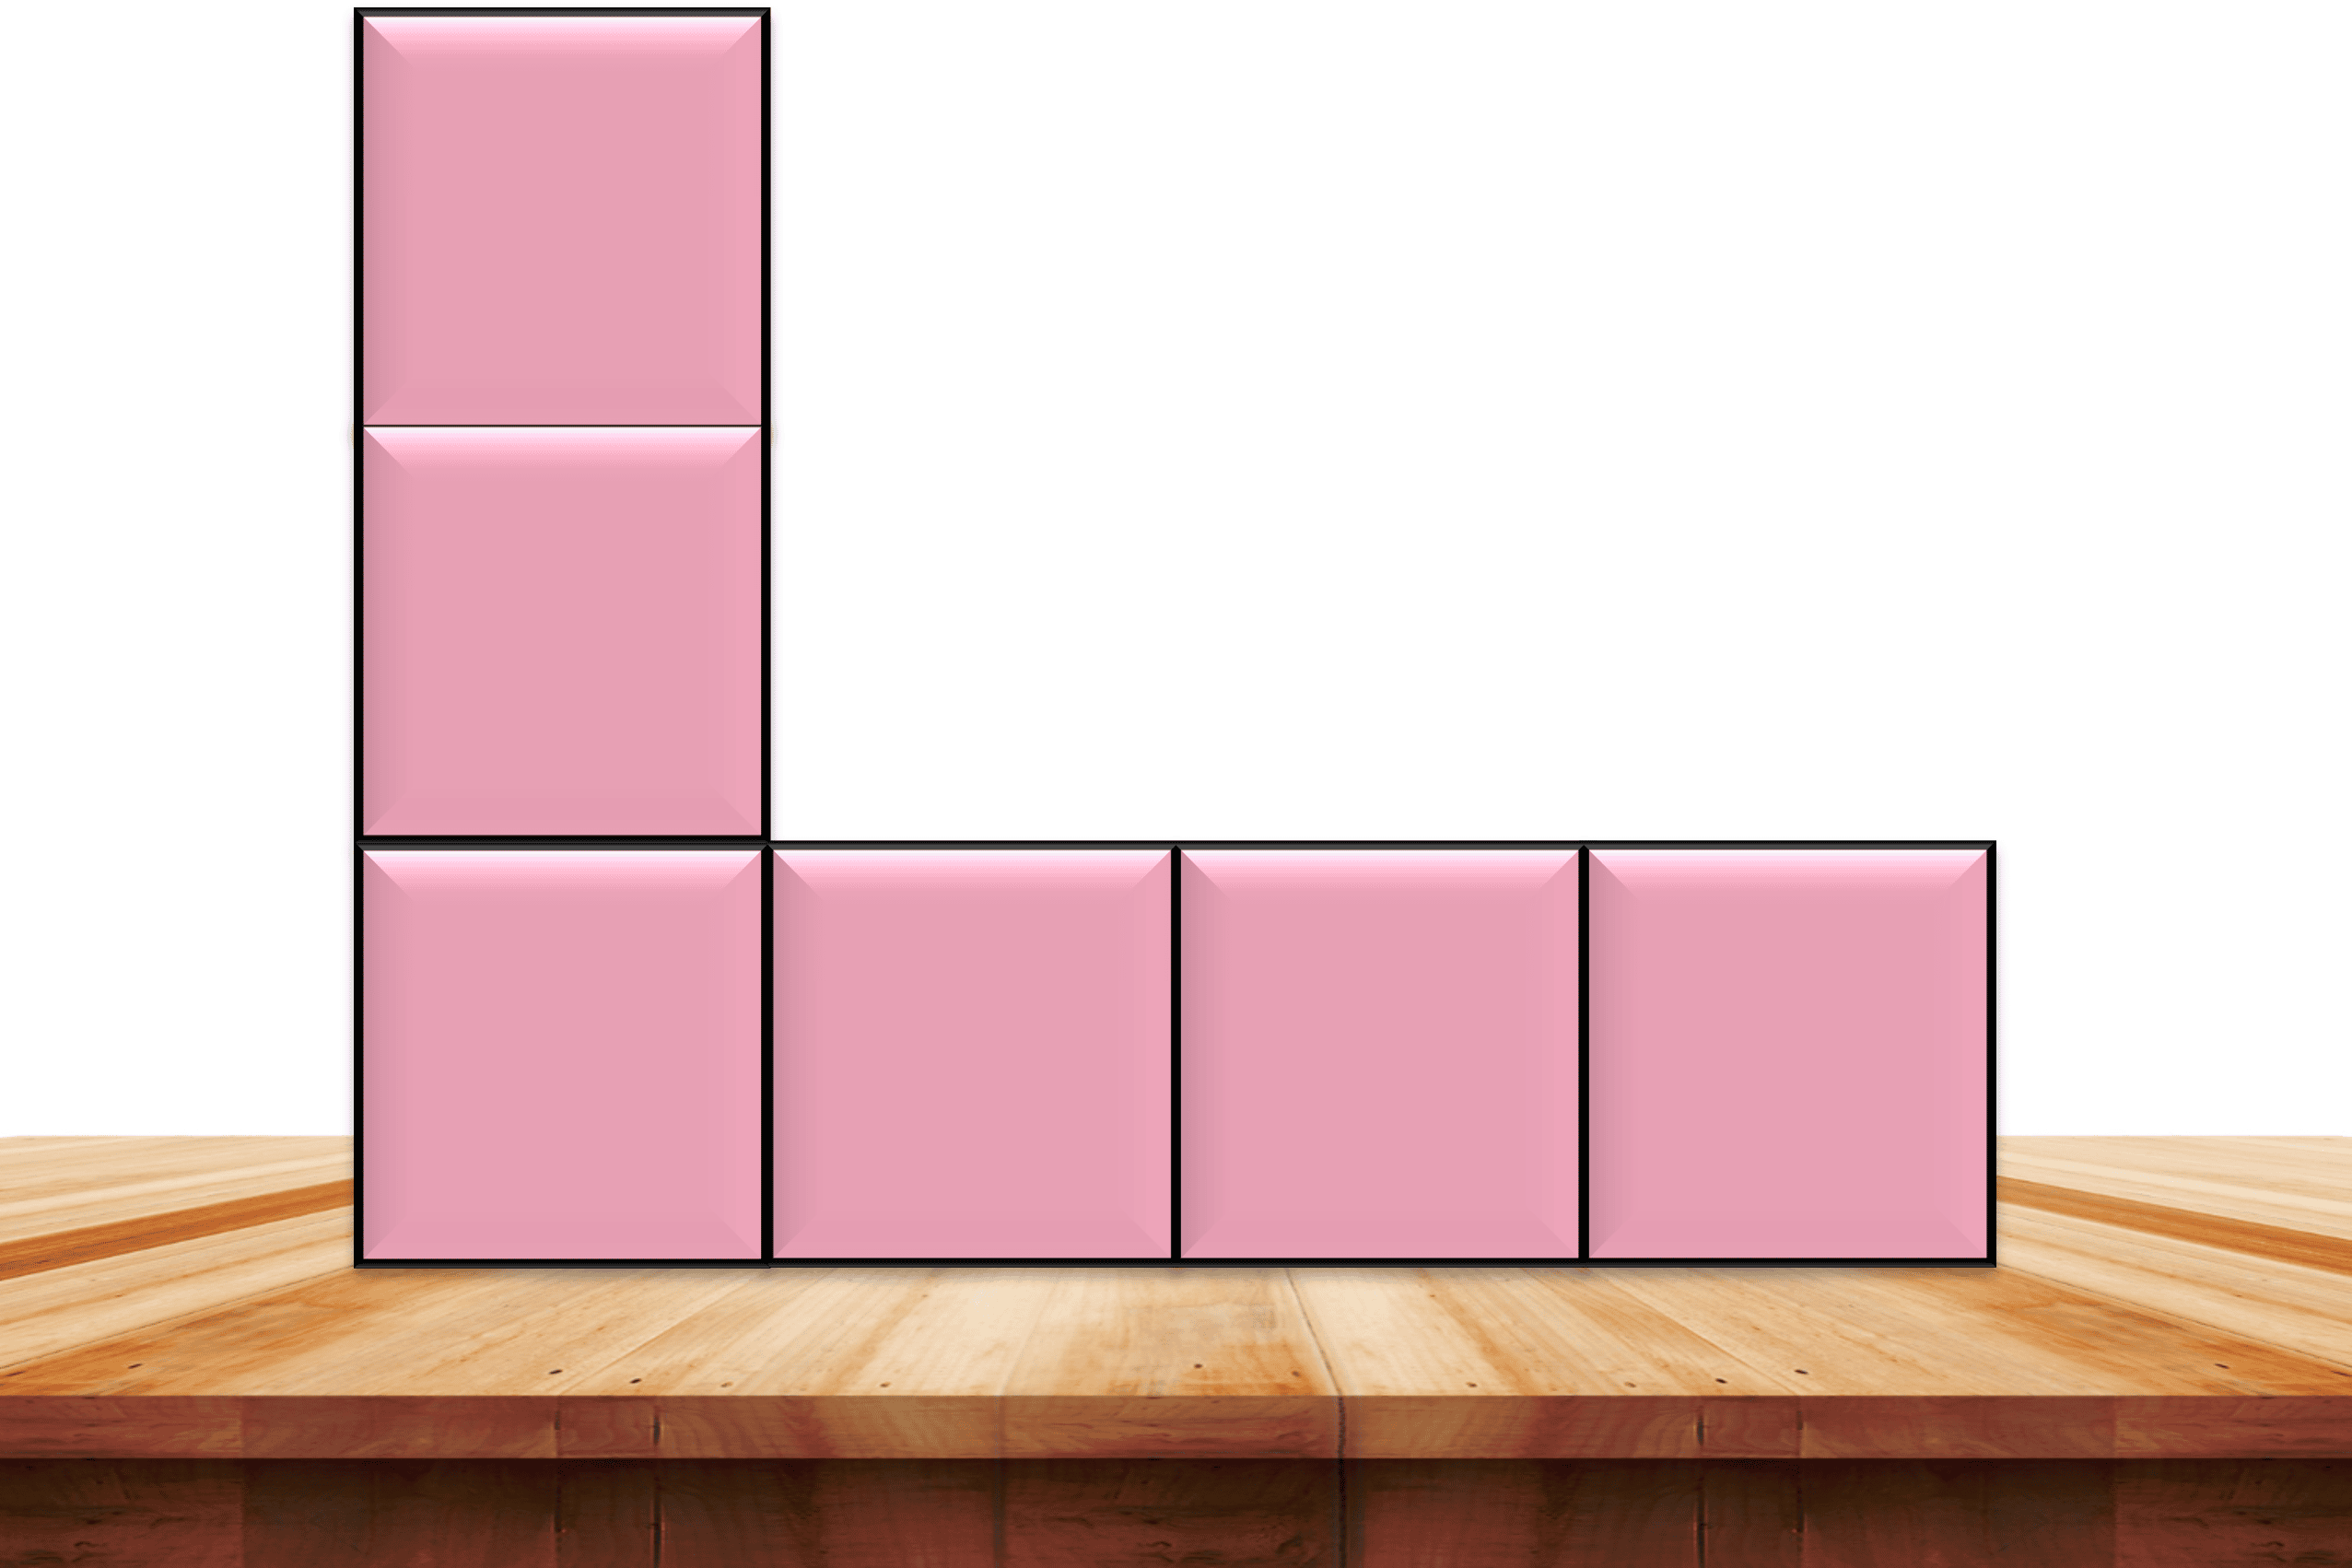
\includegraphics[width=3.5cm, height=2.5cm]{C7M14 - DT - Q5i.png}} },
  optionA={6},
  optionB={1},
  optionC={2},
  optionD={4},
  correctoption={D},
  leftmini={0.5},
  rightmini={0.4},}

\begin{minipage}{\linewidth}
\hspace{1cm}
\centering
\tiny
\renewcommand{\arraystretch}{1.25}
\begin{tabular}{|M{1.2cm}|M{0.8cm}|M{0.8cm}|M{0.8cm}|M{0.8cm}|M{0.8cm}|}
\hline
Option & A (\ding{55}) & B (\ding{55}) & C (\ding{55}) & \cellcolor{cellgreen} D (\ding{51}) & E \\ 
\hline
7 A & \highno{44\%} & \highno{13\%} & \highno{6\%} & \highred{38\%} & \highno{0\%} \\ 
 \hline 
7 B & \highno{64\%} & \highno{14\%} & \highno{7\%} & \highred{14\%} & \highno{0\%} \\ \hline
\end{tabular}
\end{minipage}

\end{frame}
% \input{4. PPT/My Answer/Math/C7/117_C7M - Q17}


\begin{frame}[shrink=0.1,label=QPC7QC7M14 - DT - Q3]{Q45 [13. Visualising Solid Shapes]}
\vspace{-0.2cm}
\mcqtextbottomOneFour{
  questionnumber={45}, 
  questionTag={C7M14 - DT - Q3}, 
  questiontext={Which will be the correct image for the given net shape?\\ \smallskip
\tikzset{every picture/.style={line width=0.75pt,scale=\scalefactor}} 
\hspace{3cm}
\begin{tikzpicture}[x=0.75pt,y=0.75pt,yscale=-1,xscale=1]
\hspace{3cm}
\draw   (205,36) -- (342,36) -- (342,63.67) -- (205,63.67) -- cycle ;
\draw   (205,63.67) -- (342,63.67) -- (342,91.34) -- (205,91.34) -- cycle ;
\draw   (205,91.34) -- (342,91.34) -- (342,119.02) -- (205,119.02) -- cycle ;
\draw   (180.43,76.65) -- (205.96,63.71) -- (205,91.34) -- cycle ;
\draw   (367.5,76.68) -- (342.9,91.31) -- (342,63.67) -- cycle ;
\end{tikzpicture} },
  optionA={{\adjustbox{scale=\scalefactor}{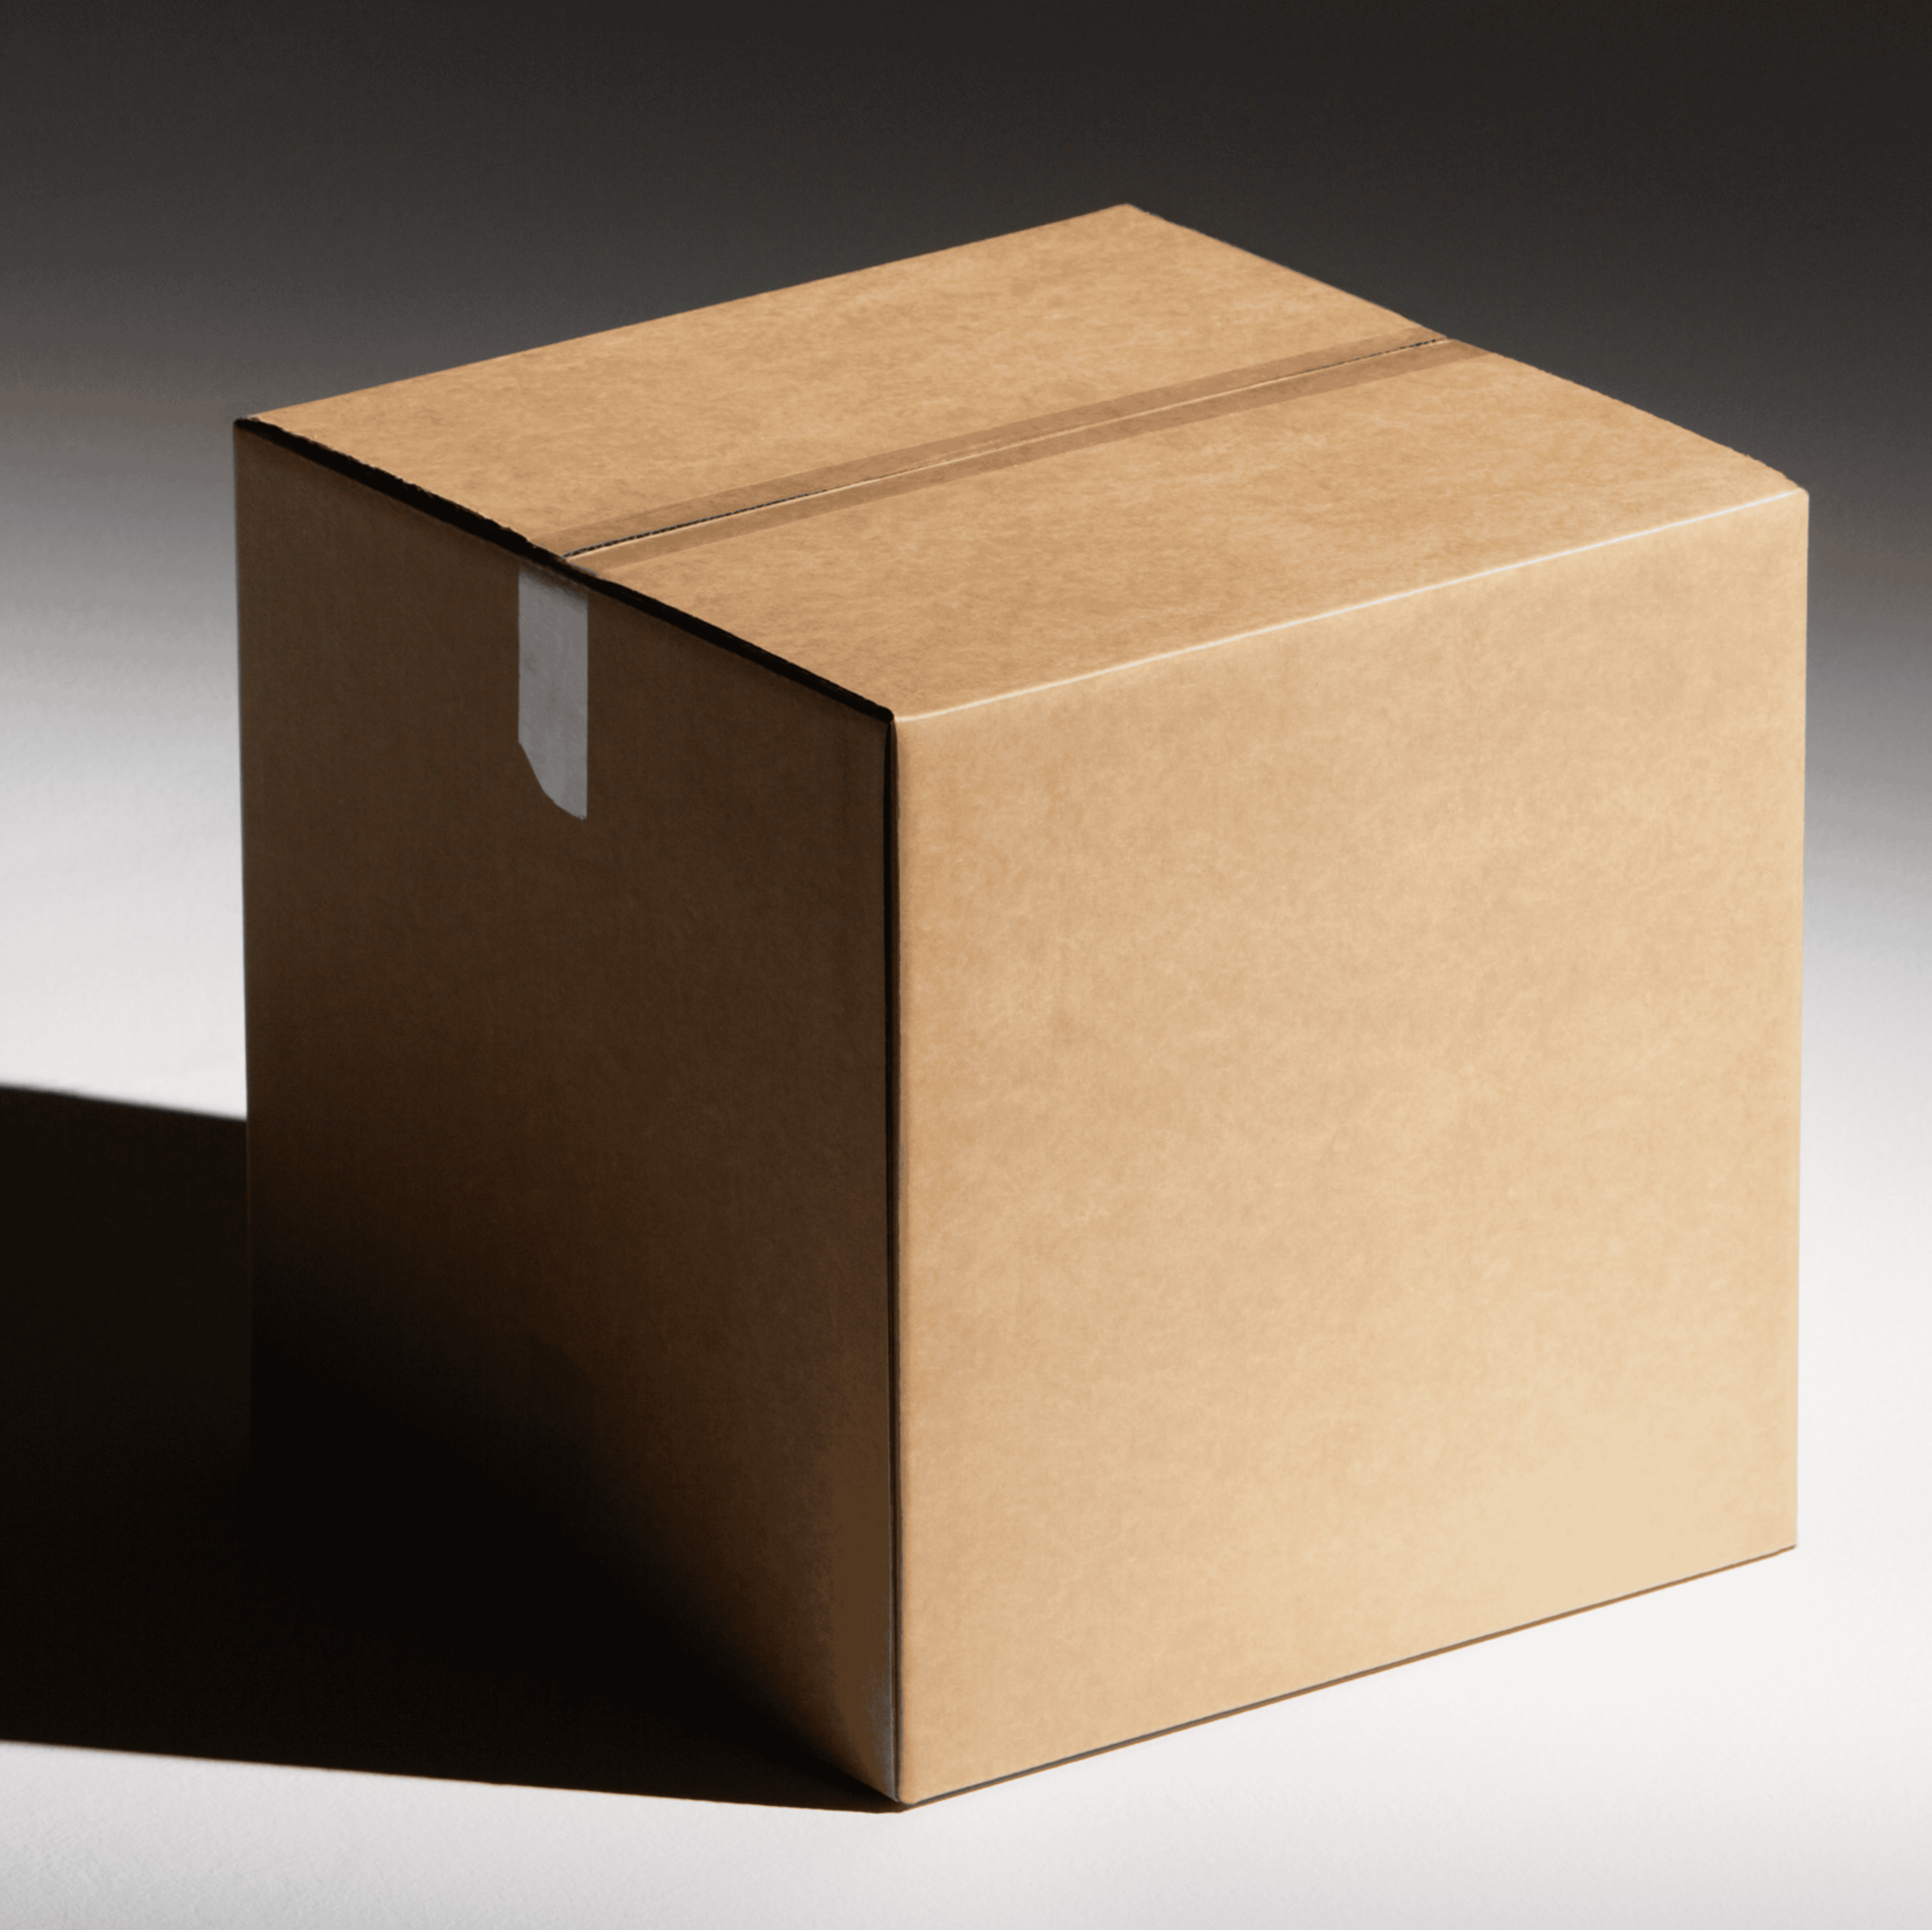
\includegraphics[width=65pt,height=55pt]{C7M14 - DT - Q3i.png }}}},
  optionB={{\adjustbox{scale=\scalefactor}{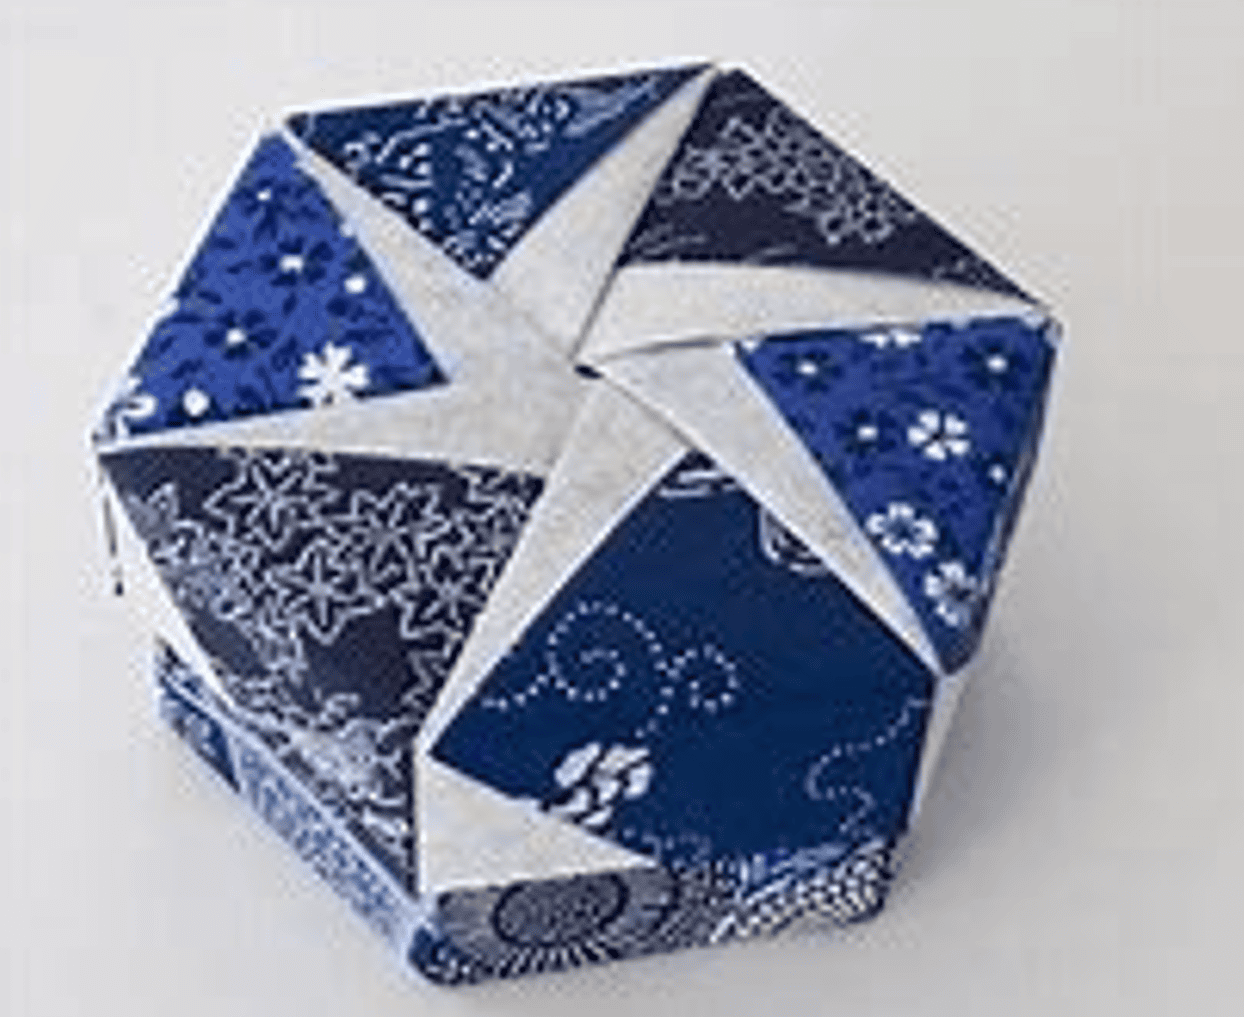
\includegraphics[width=65pt,height=55pt]{C7M14 - DT - Q3ii.png}}}},
  optionC={{\adjustbox{scale=\scalefactor}{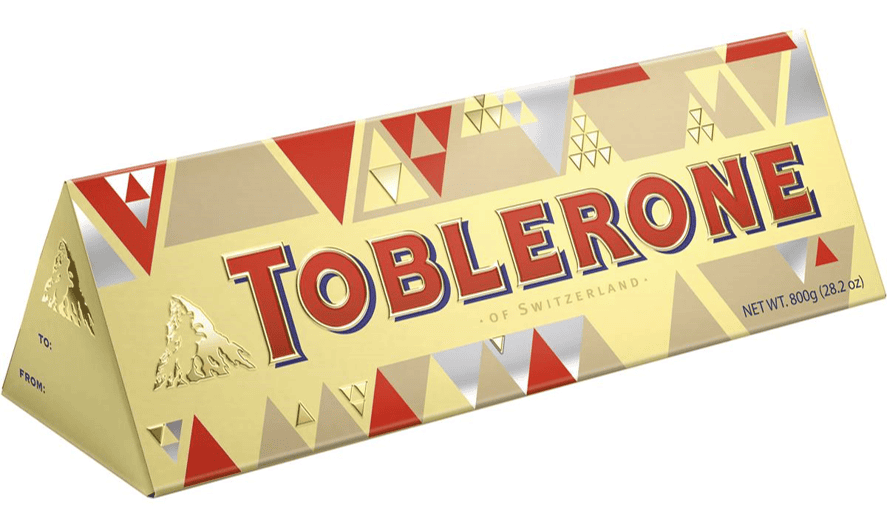
\includegraphics[width=75pt,height=55pt]{C7M14 - DT - Q34.png}}}},
  optionD={{\adjustbox{scale=\scalefactor}{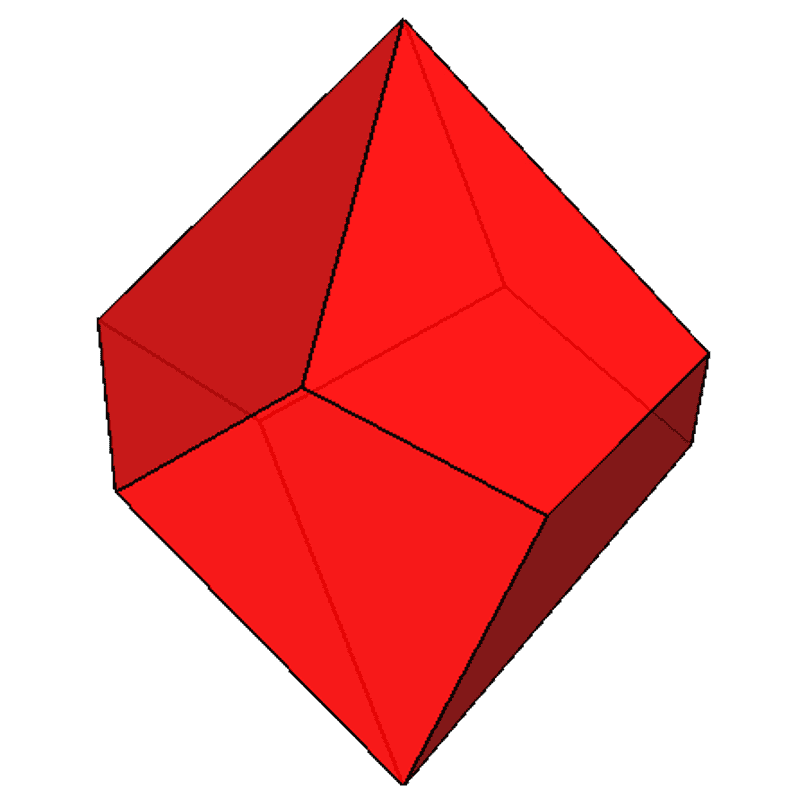
\includegraphics[width=65pt,height=55pt]{C7M14 - DT - Q3iv.png}}}},
  correctoption={C},}

\begin{minipage}{\linewidth}
\hspace{1cm}
\centering
\tiny
\renewcommand{\arraystretch}{1.25}
\begin{tabular}{|M{1.2cm}|M{0.8cm}|M{0.8cm}|M{0.8cm}|M{0.8cm}|M{0.8cm}|}
\hline
Option & A (\ding{55}) & B (\ding{55}) & \cellcolor{cellgreen} C (\ding{51}) & D (\ding{55}) & E \\ 
\hline
7 A & \highno{0\%} & \highno{0\%} & \highgreen{100\%} & \highno{0\%} & \highno{0\%} \\ 
 \hline 
7 B & \highno{0\%} & \highno{0\%} & \highgreen{100\%} & \highno{0\%} & \highno{0\%} \\ \hline
\end{tabular}
\end{minipage}

\end{frame}
% \input{4. PPT/My Answer/Math/C7/117_C7M - Q45}

%

    